
%%%%%%%%%%%%%%%%                                ~~~~~~~~~~~~~~~~~~~~~~~~~~~~~~~~~~~~~~~~~~~~~~~~~~
% CONDITIONALS %
%%%%%%%%%%%%%%%%                                ~~~~~~~~~~~~~~~~~~~~~~~~~~~~~~~~~~~~~~~~~~~~~~~~~~

\newif\ifPeerReview\PeerReviewfalse             % Whether to create the PeerReview version or
                                                % Journal version
\newif\ifFlatArchive\FlatArchivefalse           % Whether archive is flat (messy) or contain 
                                                % subfolders for graphics etc.
\newif\ifFloatAtEnd\FloatAtEndfalse             % Available in PeerReview mode:
                                                % Place floats at end of document?
\newif\ifTODO\TODOtrue                        % Use todo notes?

%%%%%%%%%%%%                                    ~~~~~~~~~~~~~~~~~~~~~~~~~~~~~~~~~~~~~~~~~~~~~~~~~~
% IEEEtran %
%%%%%%%%%%%%                                    ~~~~~~~~~~~~~~~~~~~~~~~~~~~~~~~~~~~~~~~~~~~~~~~~~~

\ifPeerReview
\documentclass[12pt,journal,captionsoff,onecolumn]{IEEEtran}
\newcommand\CLASSINPUTbaselinestretch{1.66}     % http://theoval.cmp.uea.ac.uk/~nlct/latex/thesis/node17.html
\else
\documentclass[journal]{IEEEtran}
\fi



%%%%%%%%%%%%%%%%%%%%%%%%%%%%%%                  ~~~~~~~~~~~~~~~~~~~~~~~~~~~~~~~~~~~~~~~~~~~~~~~~~~
% IEEE ''APPROVED'' PACKAGES %
%%%%%%%%%%%%%%%%%%%%%%%%%%%%%%                  ~~~~~~~~~~~~~~~~~~~~~~~~~~~~~~~~~~~~~~~~~~~~~~~~~~


\ifCLASSINFOpdf
   \usepackage[dvips]{graphicx}                 % Might not work. Use 'latex' instead of 
   \ifFlatArchive\else                          % 'pdflatex'
      \graphicspath{./gfx/}
   \fi
\else
   \usepackage[dvips]{graphicx}
   \ifFlatArchive\else
      \graphicspath{./gfx/}
   \fi
\fi

\RequirePackage[table,dvipsnames,svgnames]{xcolor}

\usepackage[cmex10]{amsmath}                    % cmex10 option to be IEEE explore compliant
\interdisplaylinepenalty=2500                   % Allows multiline equations to be broken

% \RequirePackage{amssymb}

\RequirePackage{array}

\ifCLASSOPTIONcompsoc
   \usepackage[caption=false,font=normalsize,labelfont=sf,textfont=sf]{subfig}
\else
   \usepackage[caption=false,font=footnotesize]{subfig}
\fi
\ifCLASSOPTIONcaptionsoff                       % IEEE promoted hack to turn off captions from the 
   \let\MYorigsubfloat\subfloat                 % subfloat package should the captionsoff option
   \renewcommand{\subfloat}[2][\relax]{\MYorigsubfloat[]{#2}} % be specified.
\fi

\ifFloatAtEnd
\ifCLASSOPTIONcaptionsoff                       % Places float at the end of the document when the
  \usepackage[nomarkers]{endfloat}              % captionsoff options is specified to IEEEtrans.cls
  \let\MYoriglatexcaption\caption               % (PeerReview mode)
  \renewcommand{\caption}[2][\relax]{\MYoriglatexcaption[#2]{#2}}
\fi
\fi

\usepackage{fixltx2e}                           % Fix some twocolumn float problems

%\usepackage{stfloats}                          % Allows: \begin{figure*}[!b]
                                                % (double column figures on top/bottom)

\usepackage{url}                                % Support for handling and breaking URLs

% NOTE: PDF hyperlink and bookmark features are not required in IEEE
%       papers and their use requires extra complexity and work.
\newcommand\MYhyperrefoptions{bookmarks=true,bookmarksnumbered=true,
pdfpagemode={UseOutlines},plainpages=false,pdfpagelabels=true,
colorlinks=true,linkcolor={black},citecolor={black},urlcolor={black},
pdftitle={Low Complexity Adaptive Beamformer for Active Sonar Imaging},
pdfsubject={},
pdfauthor={Jo Inge Buskenes},
pdfkeywords={adaptive beamforming, beamforming, complexity, sonar, active}}%
\ifCLASSINFOpdf
   \usepackage[\MYhyperrefoptions,pdftex]{hyperref}
\else
   \usepackage[\MYhyperrefoptions,breaklinks=true,dvips]{hyperref}
   \usepackage{breakurl}                        % Allows 'dvips' driver to break links
\fi

%%%%%%%%%%%%%%%%%%%%%%%                         ~~~~~~~~~~~~~~~~~~~~~~~~~~~~~~~~~~~~~~~~~~~~~~~~~~
% ADDITIONAL PACKAGES %       
%%%%%%%%%%%%%%%%%%%%%%%                         ~~~~~~~~~~~~~~~~~~~~~~~~~~~~~~~~~~~~~~~~~~~~~~~~~~

\newcounter{todoidx}
% \setcounter{todoidx}

\ifTODO
   \definecolor{todobackground}{rgb}{0.95,0.95,0.95}
   \setlength\marginparsep{3pt}
   \setlength\marginparwidth{42pt}
   \newlength\marginparwidthsmall
   \setlength\marginparwidthsmall{\marginparwidth}
   \addtolength\marginparwidthsmall{-7pt}
   \newcommand\todo[1]{%
      \addtocounter{todoidx}{1}%
      {\color{Red}\fbox{\bf\thetodoidx{}}}%
      \marginpar{%
         {\vspace*{-10pt}\color{Red}\fbox{\bf\thetodoidx{}}}\\%
         \fcolorbox{red}{todobackground}{\parbox{\marginparwidthsmall}{#1}}}}

   \newcommand\todopar[1]{\fcolorbox{red}{white}{\parbox{0.97\linewidth}{#1}}}
\else
%    \usepackage[disable]{./todonotes} 
   \newcommand\todo[1]{}
\fi

\newenvironment{narrow}[2]{%
\begin{list}{}{%
\setlength{\topsep}{0pt}%
\setlength{\leftmargin}{#1}%
\setlength{\rightmargin}{#2}%
\setlength{\listparindent}{\parindent}%
\setlength{\itemindent}{\parindent}%
\setlength{\parsep}{\parskip}}%
\item[]}{\end{list}}

%%%%%%%%%%                                      ~~~~~~~~~~~~~~~~~~~~~~~~~~~~~~~~~~~~~~~~~~~~~~~~~~
% MACROS %       
%%%%%%%%%%                                      ~~~~~~~~~~~~~~~~~~~~~~~~~~~~~~~~~~~~~~~~~~~~~~~~~~


\newcommand\Grey[1]{{\color{Grey}#1}}
\newcommand\Red[1]{{\color{Red}#1}}
\newcommand\Blue[1]{{\color{Blue}#1}}
\newcommand\DarkBlue[1]{{\color{DarkBlue}#1}}
\newcommand\LightBlue[1]{{\color{LightBlue}#1}}
\newcommand\Brown[1]{{\color{Brown}#1}}
\newcommand\Green[1]{{\color{Green}#1}}
\newcommand\SeaGreen[1]{{\color{SeaGreen}#1}}
\newcommand\Yellow[1]{{\color{yellow}#1}}
\newcommand\Orange[1]{{\color{orange}#1}}

\newcommand\nn{\nonumber\\}

\newcommand\nmat[1]{\begin{matrix}#1\end{matrix}}
\newcommand\bmat[1]{\begin{bmatrix}#1\end{bmatrix}}
\newcommand\case[1]{\begin{cases}#1\end{cases}}
\newcommand\textbox[2]{\footnotesize\text{\parbox{#1}{\centering\emph{#2}}}}

\newcommand\rand{\text{rand}}
\newcommand\randn{\text{randn}}
\newcommand\rect{\text{rect}}
\newcommand\sinc{\text{sinc}}
\newcommand\tr{\text{tr}}
\newcommand\adj{\text{adj}}

% \newcommand\max{\text{max}}
\newcommand\argmin{\text{argmin}}

\newcommand\qqquad{\quad\qquad}
\newcommand\qqqquad{\qquad\qquad}

\renewcommand\l[1]{\left#1}
\renewcommand\r[1]{\right#1}

% {\text{\parbox{1.5cm}{\centering volume hyper- sphere}}}

%Keyword colouring:
\newcommand\kw[1]{#1}
\newcommand\parm[1]{#1}%\color{Black}#1\color{Black}}

\newcommand\of[1]{\scriptstyle(\parm{#1})\displaystyle}
\newcommand\df[1]{\scriptstyle[\parm{#1}]\displaystyle}
\newcommand\var[3]{#1_\text{#2}\of{#3}}

\newcommand\diag{\text{diag}}

% \raisebox{lift}[extend-above-baseline][extend-below-baseline]{text}
\newcommand\mt[1]{\text{\emph{#1}}} %mt = mathtext
\newcommand\mathnorm{\textstyle}
\newcommand\mathbig[1]{\displaystyle#1\mathnorm}
\newcommand\mathsmall[1]{\scriptstyle#1\mathnorm}
\newcommand\mathtiny[1]{\scriptscriptstyle#1\mathnorm}
\newcommand\sfrac[2]{\scriptstyle\raisebox{0.25pt}[0pt][0pt]{$\frac{#1}{#2}$}\mathnorm}
\newcommand\nfrac[2]{\textstyle\frac{#1}{#2}\displaystyle}

\newcommand\sumu[1]{\sum\limits^{#1}\,}
\newcommand\suml[1]{\sum\limits_{#1}\,}
\newcommand\sumb[2]{\sum\limits_{#1}^{#2}\,}

\newcommand\produ[1]{\prod\limits^{#1}\,}
\newcommand\prodl[1]{\prod\limits_{#1}\,}
\newcommand\prodb[2]{\prod\limits_{#1}^{#2}\,}

%Math macros:
\newcommand\diff[2]{\frac{\kw{d}\,\textstyle #1\scriptstyle}{\kw{d\parm{#2}}}\displaystyle}
\newcommand\ddiff[2]{\frac{\kw{d^2}\,\displaystyle #1\scriptstyle}{\kw{d\parm{#2}}^2}\displaystyle}

\renewcommand\d[1]{\scriptstyle\kw{\,d\parm{#1}}\displaystyle}

% These commands are mutually exclusive. Remember to "renew" in v2.
\newcommand\intb[4]{\int\limits_{#3}^{#4} #1 \d{#2}} % \int{exp}{var}{from}{to}
\newcommand\intl[3]{\int\limits_{#3} #1 \d{#2}} % \int{exp}{var}{for all}
\newcommand\intu[2]{\int #1 \d{#2}} % \int{exp}{var}{for all}

\newcommand\T{^{\scriptscriptstyle T}}
\renewcommand\H{^{\scriptscriptstyle H}}

\renewcommand\vec[1]{\boldsymbol{#1}}
\newcommand\mat[1]{\boldsymbol{#1}}


\renewcommand*\a{\vec a}
\renewcommand*\i{\vec i}
\renewcommand*\k{\vec k}
\newcommand*\n{\vec n}
\newcommand*\p{\vec p}
\newcommand*\s{\vec s}
\newcommand*\w{\vec w}
\newcommand*\x{\vec x}
\newcommand*\y{\vec y}

\newcommand*\A{\mat A}
\newcommand*\B{\mat B}
\newcommand*\C{\mat C}
\newcommand*\E{\mat E}
% \renewcommand*\H{\mat H}
\renewcommand*\P{\mat P}
\newcommand*\eP{\mat{\hat P}}
\newcommand*\R{\mat R}
\newcommand*\Ri{\R^{-1}}
\newcommand*\eR{\mat{\hat R}}
\newcommand*\W{\mat W}
\newcommand*\X{\mat X}
\newcommand*\Xd{\X_{\!\Delta}}
\newcommand*\Y{\mat Y}

\renewcommand*\L{\mat \Lambda}
\newcommand*\U{\mat U}
% \renewcommand*\t{\mathtiny{^T}}
% \newcommand*\h{\mathtiny{^H}}
\renewcommand*\t{^T}
\newcommand*\h{^H}

\newcommand\D{\vec\nabla} %Del: Vector differential operator - nabla
\newcommand\Dx{\vec\nabla\times}
\newcommand\Dd{\vec\nabla\cdot}

\usepackage{tikz}
\usetikzlibrary{shapes,snakes}
\usepackage{amsmath,amssymb}

\newenvironment{outline}
{\begin{itemize}}
{\end{itemize}}

%    \definecolor{todobackground}{rgb}{0.95,0.95,0.95}
%    \setlength\marginparsep{3pt}
%    \setlength\marginparwidth{42pt}
%    \newlength\marginparwidthsmall
%    \setlength\marginparwidthsmall{\marginparwidth}
%    \addtolength\marginparwidthsmall{-7pt}
%    \newcommand\todo[1]{%
%       \addtocounter{todoidx}{1}%
%       {\color{Red}\fbox{\bf\thetodoidx{}}}%
%       \marginpar{%
%          {\vspace*{-10pt}\color{Red}\fbox{\bf\thetodoidx{}}}\\%
%          \fcolorbox{red}{todobackground}{\parbox{\marginparwidthsmall}{#1}}}}
% 

% correct bad hyphenation here
% \hyphenation{op-tical net-works semi-conduc-tor}


%%%%%%%%%%%%%%%%%%                              ~~~~~~~~~~~~~~~~~~~~~~~~~~~~~~~~~~~~~~~~~~~~~~~~~~
% DOCUMENT START %
%%%%%%%%%%%%%%%%%%                              ~~~~~~~~~~~~~~~~~~~~~~~~~~~~~~~~~~~~~~~~~~~~~~~~~~

% \RequirePackage[utf8]{inputenc}%              % Set input encoding (optionally latin1)
% \RequirePackage[T1]{fontenc}%                 % Set font encoding


\begin{document}

\title{Low Complexity Adaptive Beamformer\\ for Active Sonar Imaging}

\author{Jo~Inge~Buskenes, %
        Andreas~Austeng, %
        Carl-Inge~Columbo~Nilsen%
\IEEEcompsocitemizethanks{\IEEEcompsocthanksitem All authors are with the Department
of Informatics, University of Oslo, Norway.}% <-this % stops a space

% \thanks{Manuscript received April 19, 2005; revised January 11, 2007.}
}

% The paper headers
\markboth{IEEE Journal of Oceanic Engineering}%
{Low Complexity Adaptive Beamformer for Active Sonar Imaging}

% Publishers ID mark:
%\IEEEpubid{0000--0000/00\$00.00~\copyright~2007 IEEE}

% use for special paper notices
%\IEEEspecialpapernotice{(Invited Paper)}

% for Computer Society papers, we must declare the abstract and index terms
% PRIOR to the title within the \IEEEcompsoctitleabstractindextext IEEEtran
% command as these need to go into the title area created by \maketitle.
\IEEEcompsoctitleabstractindextext{%
\begin{abstract}

\begin{itemize}
\item Dynamic weights $\Rightarrow$ greater contrast/resolution potential
\item But:
\begin{itemize}
\item Active system $\Rightarrow$ noise and signal correlated $\Rightarrow$ adaptive beamformers no longer robust.
\item Subarray averaging decorrelate the noise, but in the process we sacrifice resolution.
\item Computationally complex O($M^3$) due to inversion of a spatial covariance matrix. LCA is only O($MW$). Even if Capon subspace/beamspace versions exist, they remain more complex than the LCA, and is not as ideally suited for implementation of SIMD hardware (GPUs, DSPs, ...).
\end{itemize}
\item LCA is inherently robust, is ``parameter free'' once setup with a well designed window set, and can often be implemented with minor modifications to already existing DAS beamformers.
\end{itemize}

\end{abstract}

% Keywords (normally not used for peer reviews)
\ifPeerReview\else
\begin{IEEEkeywords}
Beamforming, adaptive beamforming, sonar, active, complexity.
\end{IEEEkeywords}
\fi}
% \fi

% make the title area
\maketitle

% This command fixes abstract positioning for compsoc articles:
\IEEEdisplaynotcompsoctitleabstractindextext

% (Optional) Add some extra info on cover page of peer review papers:
% \ifCLASSOPTIONpeerreview
% \begin{center} \bfseries EDICS Category: 3-BBND \end{center}
% \fi

% Insert page break and insert second title (peer review mode)
\IEEEpeerreviewmaketitle



\section{Introduction}


\begin{itemize}
\item Sell it!
\item As briefly as possible, introduce beamforming.
\item Adaptive beamformer's potential lies in its ability to suppress interference power
\item Why adaptive beamformers struggle in active sonar systems. Correlated noise, robustification kills the adaptive potential. Quite computationally intensive. Constraints must be applied in one way or another - parameters must be tuned.
\begin{itemize}
\item Noise and signal is correlated. Spatial averaging required. 
\item Increases variance of speckle (not only in active systems?), spatial compunting \cite{Vignon2009} (US) or time averaging?. Subarray averaging applied here \cite{Synnevag2007} (US) \todo{Is it bad to mix ultrasound/ sonar refs?}
\end{itemize}
\item LCA is like DAS, only we test several windows and choose the one that yield the lowest beamformer output power. Ultrasound \cite{Synnevag2008}, active sonar \cite{Buskenes2011}\cite{Blomberg2011}\cite{Blomberg2012}\todo{who was that guy in the 80ties?}
\item Outline: 
\begin{itemize}
\item Methods.
\item See what happens to Capon's response %\cite{Synnevag2007}  when means for robustification are added.
\item Setup the window set for LCA to match this.
\item Notice that the LCA performs like Capon, even with a small window database.
\item Start with Kaiser, see that other window functions also work well.
\end{itemize}
\end{itemize}
\todopar{Out of the blue idea: Weigh CF with LCA? This guy did it with MVDR \cite{Wang2009}. Probably you know already... Okay, back on track.}


\section{Methods}

\todopar{Threw some formulas in to get a feel of them}

\begin{align}
z[n] = \sumb{m=0}{M-1} w_m[n]^*x_m[n-\Delta_m] = \w\H[n]\Xd[n]
\end{align}
where
\begin{align}
\w[n] = \bmat{w_0[n]\\w_1[n]\\\vdots\\w_{M-1}[n]} \quad \text{and} \quad\Xd[n] = \bmat{x_0[n]\\x_1[n]\\\vdots\\x_{M-1}[n]}.
\end{align}

Minimum variance distortionless resonse \cite{Capon1969}
\begin{align}
\underset{\w[n]}{\argmin}\, E\{ |z[n]|^2 \} = \underset{\w[n]}{\argmin}\, \w\H[n]\R[n]\w[n], 
\end{align}
subject to
\begin{align}
\w\H[n]\a = 1,
\end{align}
where
\begin{align}
\R[n] = E\{ \x\x\H \}.
\end{align}
If $\eR$ is the estimate of $\R$, the solution to the MVDR beamformer is
\begin{gather*}
\vec w[n] = \frac{\hat{\mat R}\,\!^{-1}[n]\vec a}{\vec a\H\hat{\mat R}\,\!^{-1}[n]\vec a} = \frac{\text{\raisebox{1.9pt}{$\vec\chi$}}[n]}{\vec a\H\text{\raisebox{1.9pt}{$\vec\chi$}}[n]}
\end{gather*}
A robust estimate of $\eR$ is found by
\begin{itemize}
\item Spatial averaging to decorrelate noise from signal. \emph{Subarray averaging} used here.
\item Temporal averaging to ensure valid speckle statistics.
\item \emph{Diagonal loading} to ensure  numerical stability prior to inversion.
\item Choice of robustification parameters \cite{Synnevag2007}
\end{itemize}

Here $\vec a$ is a \emph{steering vector} that if set to $\vec 1$ steers towards broadside, and $\hat{\mat R}$ is an estimate of the spatial covariance matrix, often computed as
\begin{gather*}
r_{ij}[n] = \frac{1}{K(2N_{\text{avg}}+1)}\sumb{k=0}{K-1} \sumb{n'=n-N_{\text{avg}}}{n+N_{\text{avg}}} x_{i+k}[n']\,x_{j+k}[n'],
\end{gather*}
where $r_{ij}$ is the $(i,j)$'th element of the covariance matrix, $K$ is the number of subarrays, $2N_{\text{avg}}+1$ is the number of samples to perform time averaging over, and $\vec x_i[n']$ is the data recorded by the $i$'th sensor at sample $n'$. 

\emph{Diagonal loading} chosen as \cite{Synnevag2007}
\begin{align}
\varepsilon = \Delta \cdot \tr\{\eR[n]\}
\end{align}

\section{Results}

% \begin{figure}[!t]\centering
% % \includegraphics[width=2.5in]{}
% \caption{Simulation Results}
% \label{fig_sim}
% \end{figure}

\newpage
\begin{figure*}[!t]
\begin{narrow}{-1.2cm}{-1.2cm}\centering\vspace{-1.0cm}
\textbf{1. LCA with trigonometric and Kaiser windows - Capon shining}\\
\begin{tabular}[c]{l l l l}
\bf General & M = 32                            & $\Delta r = \frac{c}{2B}$ = 2.5 cm & $\frac{640\,\text{pixels}] / 12\,\text{m}}{\Delta r} = \frac{4}{3}$ \\
\bf LCA     & $\beta \in [0,10]$ (9 values) & $\phi \in [-1.07,1.07]$ deg (9 values) & Navg = 3 \\
\bf Capon   & $\Delta$ = 0.01                 & L = 16                           & Navg = 3 \\
\end{tabular}
\subfloat[LCA Window Response]{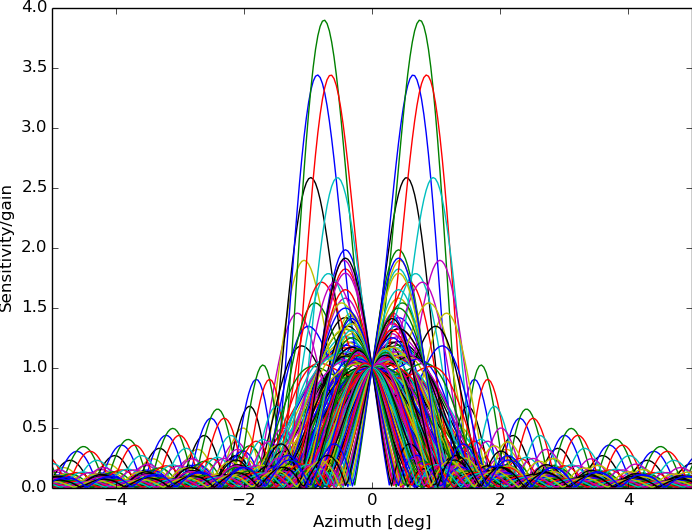
\includegraphics[width=0.49\linewidth]{gfx/1_window_response.png}}\hfill
\subfloat[Mean images]{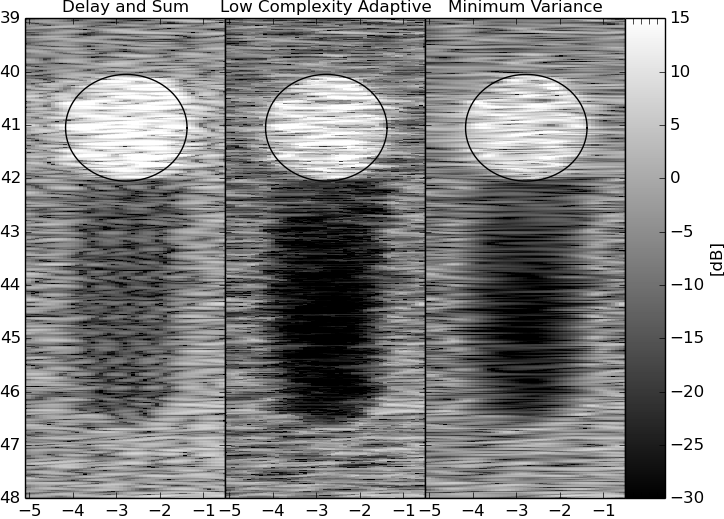
\includegraphics[width=0.49\linewidth]{gfx/1_mean_imgs.png}}\\
\subfloat[Windows ($\beta$)]{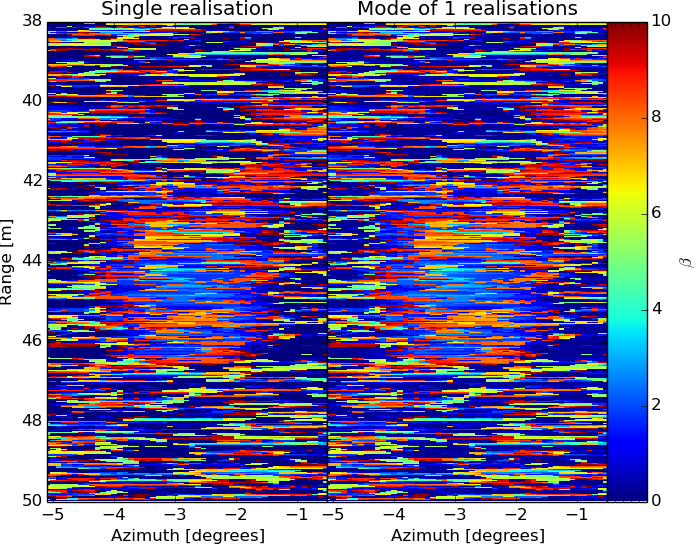
\includegraphics[width=0.49\linewidth]{gfx/1_windows_beta.png}}\hfill
\subfloat[Windows ($\phi$)]{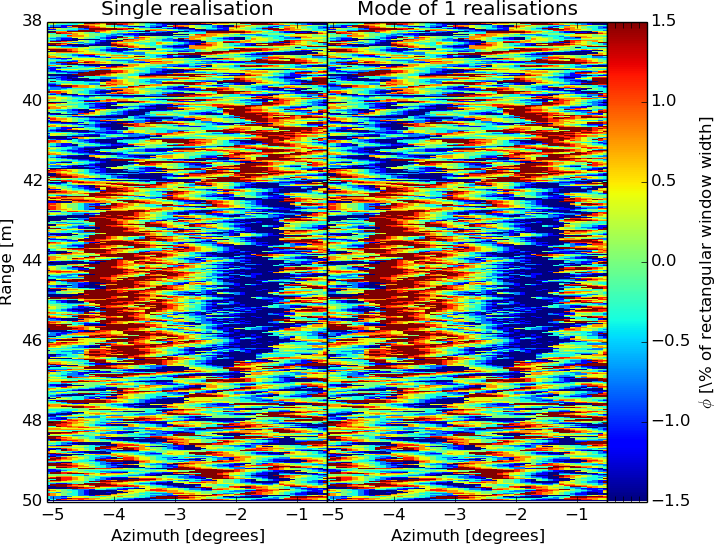
\includegraphics[width=0.48\linewidth]{gfx/1_windows_phi.png}}\\
\subfloat[Capon win. resp. through shadow]{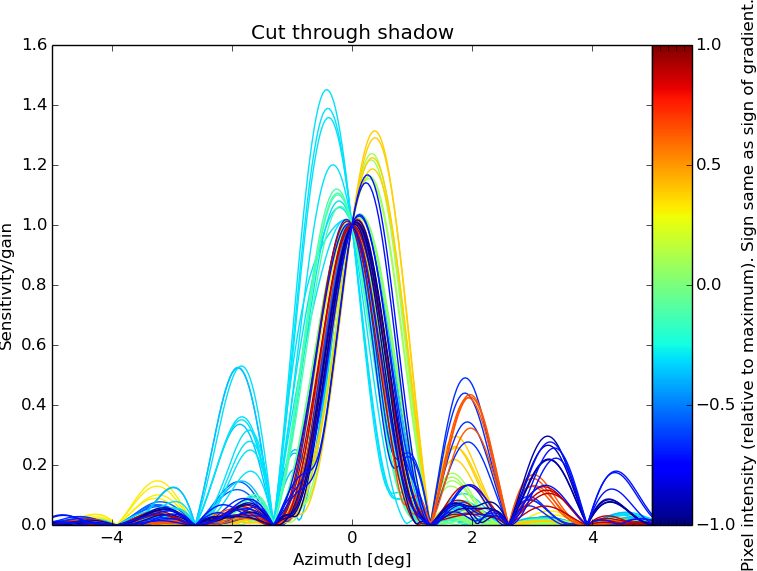
\includegraphics[width=0.49\linewidth]{gfx/1_win_resp_cut_shadow.png}}\hfill
\subfloat[Capon win. resp. through highlight]{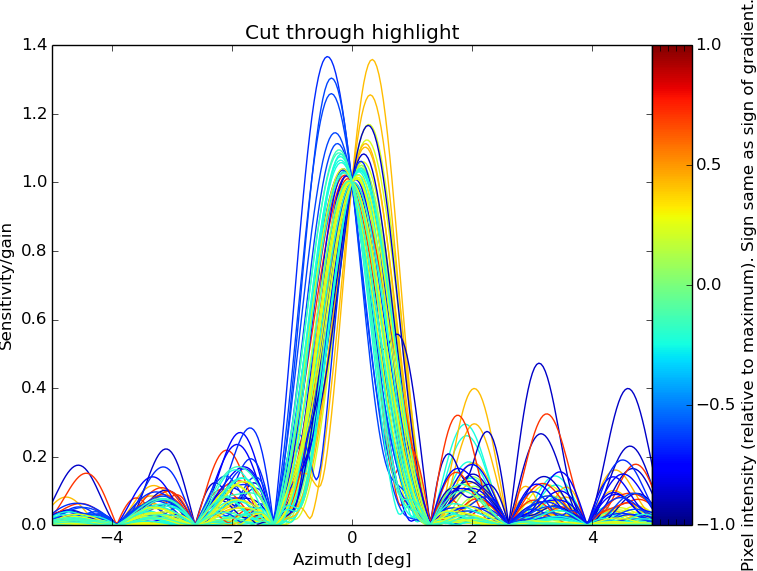
\includegraphics[width=0.49\linewidth]{gfx/1_win_resp_cut_highlight.png}}\\
\end{narrow}
\end{figure*}
\newpage
\begin{figure*}[!t]
\begin{narrow}{-1.2cm}{-1.2cm}\centering\vspace{-1.0cm}
\textbf{2. Capon: Tuning regularisation.}\\
\begin{tabular}[c]{l l l l}
\bf General & M = 32                            & $\Delta r = \frac{c}{2B}$ = 2.5 cm & $\frac{640\,\text{pixels}] / 12\,\text{m}}{\Delta r} = \frac{4}{3}$ \\
\bf LCA     & $\beta \in [0,10]$ (9 values) & $\phi \in [-1.07,1.07]$ deg (9 values) & Navg = 3 \\
\bf Capon   & $\Delta$ = 0.05                 & L = 16                           & Navg = 3 \\
\end{tabular}
\subfloat[LCA Window Response]{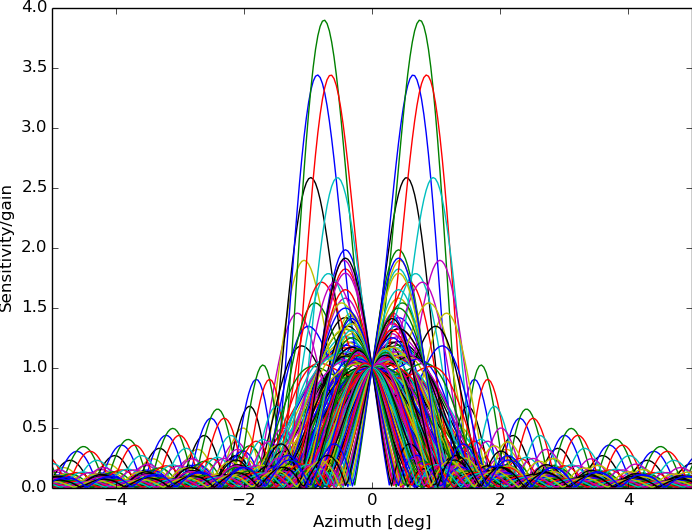
\includegraphics[width=0.49\linewidth]{gfx/2_window_response.png}}\hfill
\subfloat[Mean images]{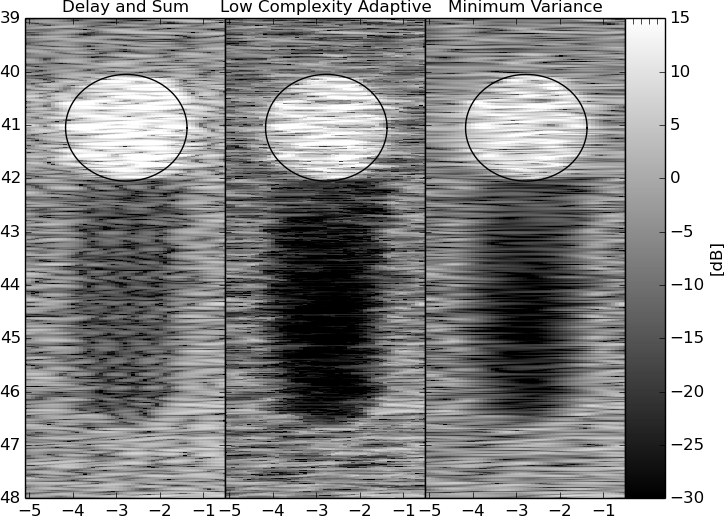
\includegraphics[width=0.49\linewidth]{gfx/2_mean_imgs.png}}\\
\subfloat[Windows ($\beta$)]{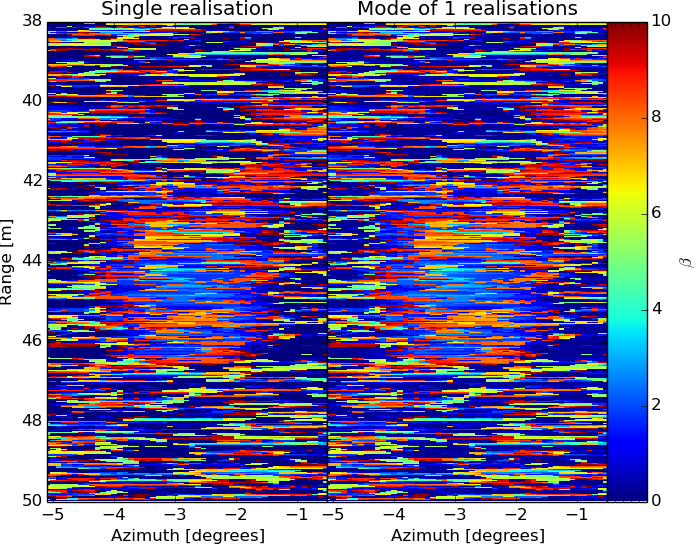
\includegraphics[width=0.49\linewidth]{gfx/2_windows_beta.png}}\hfill
\subfloat[Windows ($\phi$)]{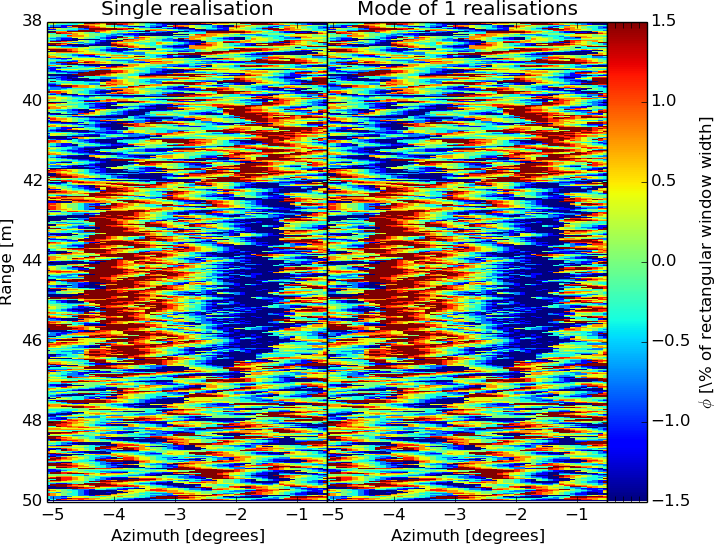
\includegraphics[width=0.48\linewidth]{gfx/2_windows_phi.png}}\\
\subfloat[Capon win. resp. through shadow]{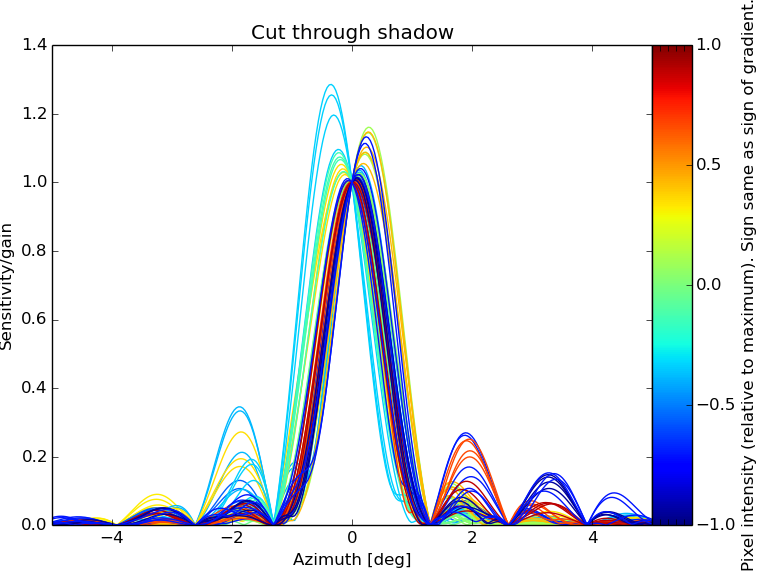
\includegraphics[width=0.49\linewidth]{gfx/2_win_resp_cut_shadow.png}}\hfill
\subfloat[Capon win. resp. through highlight]{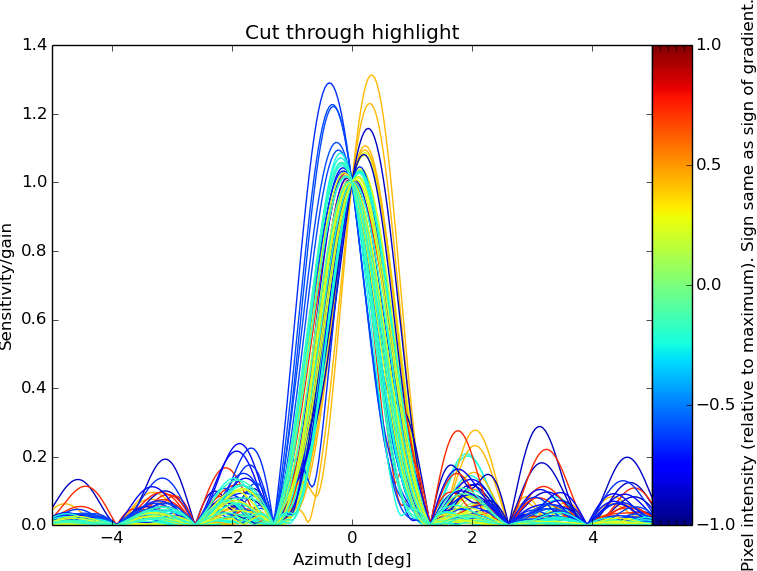
\includegraphics[width=0.49\linewidth]{gfx/2_win_resp_cut_highlight.png}}\\
\end{narrow}
\end{figure*}
\newpage
\begin{figure*}[!t]
\begin{narrow}{-1.2cm}{-1.2cm}\centering\vspace{-1.0cm}
\textbf{3. Capon: Tuning regularisation.}\\
\begin{tabular}[c]{l l l l}
\bf General & M = 32                            & $\Delta r = \frac{c}{2B}$ = 2.5 cm & $\frac{640\,\text{pixels}] / 12\,\text{m}}{\Delta r} = \frac{4}{3}$ \\
\bf LCA     & $\beta \in [0,10]$ (9 values) & $\phi \in [-1.07,1.07]$ deg (9 values) & Navg = 3 \\
\bf Capon   & $\Delta$ = 0.20                 & L = 16                           & Navg = 3 \\
\end{tabular}
\subfloat[LCA Window Response]{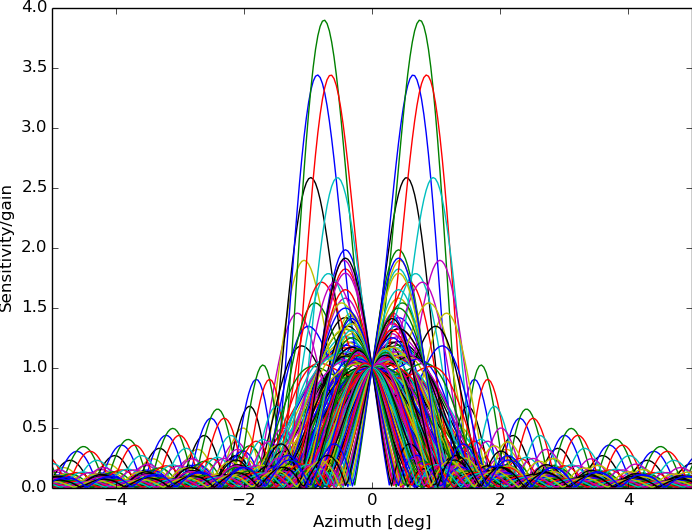
\includegraphics[width=0.49\linewidth]{gfx/3_window_response.png}}\hfill
\subfloat[Mean images]{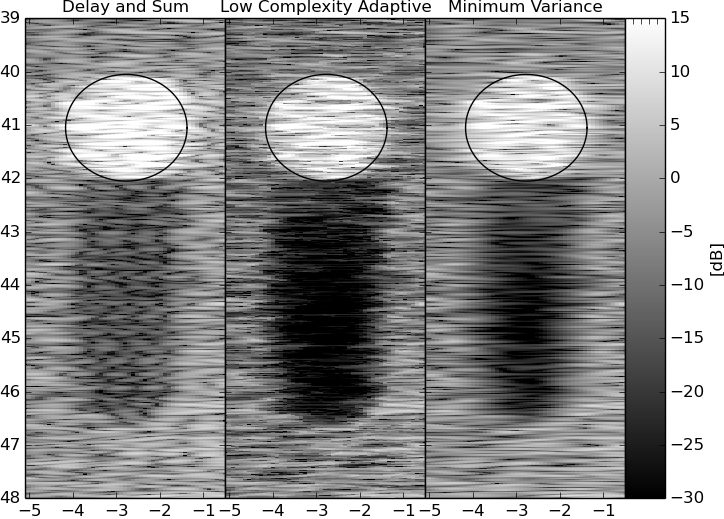
\includegraphics[width=0.49\linewidth]{gfx/3_mean_imgs.png}}\\
\subfloat[Windows ($\beta$)]{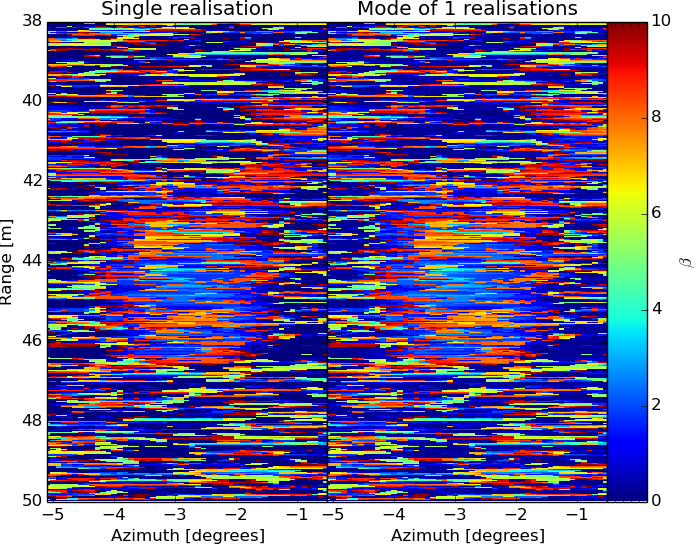
\includegraphics[width=0.49\linewidth]{gfx/3_windows_beta.png}}\hfill
\subfloat[Windows ($\phi$)]{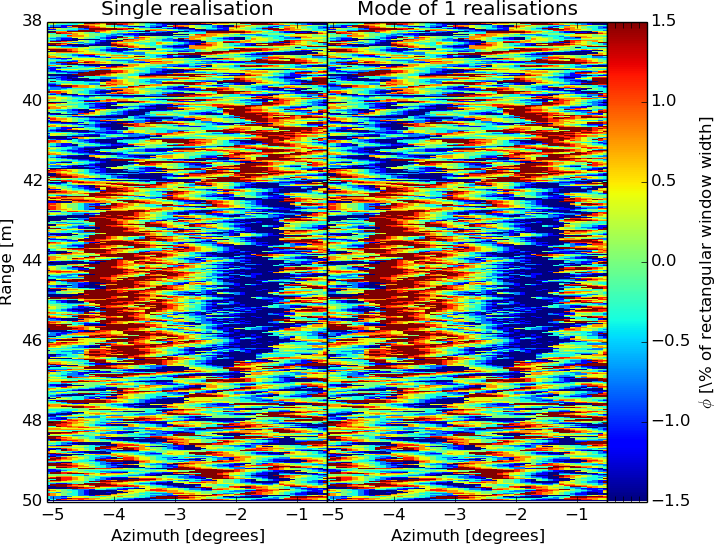
\includegraphics[width=0.48\linewidth]{gfx/3_windows_phi.png}}\\
\subfloat[Capon win. resp. through shadow]{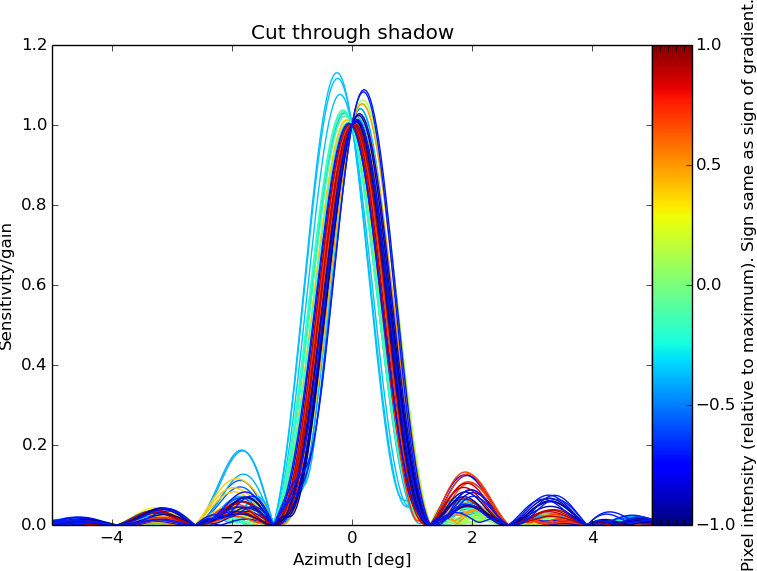
\includegraphics[width=0.49\linewidth]{gfx/3_win_resp_cut_shadow.png}}\hfill
\subfloat[Capon win. resp. through highlight]{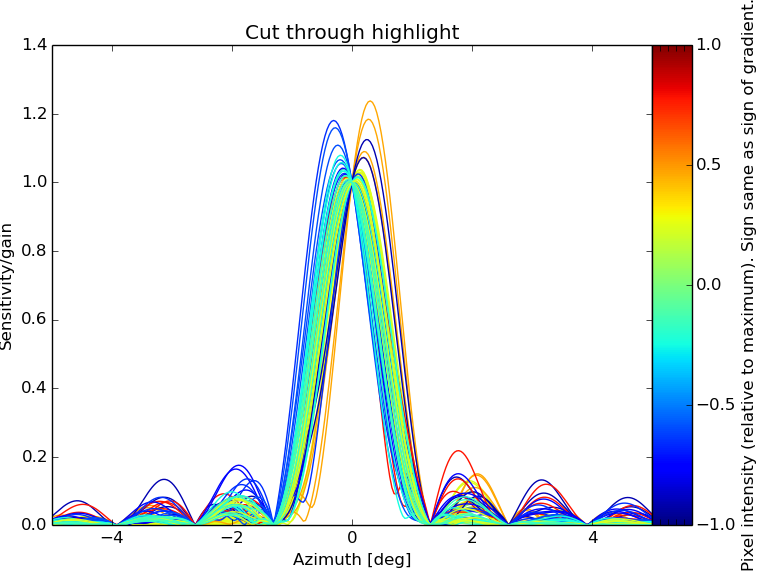
\includegraphics[width=0.49\linewidth]{gfx/3_win_resp_cut_highlight.png}}\\
\end{narrow}
\end{figure*}
\newpage
\begin{figure*}[!t]
\begin{narrow}{-1.2cm}{-1.2cm}\centering\vspace{-1.0cm}
\textbf{4. Capon: Tuning subarray.}\\
\begin{tabular}[c]{l l l l}
\bf General & M = 32                            & $\Delta r = \frac{c}{2B}$ = 2.5 cm & $\frac{640\,\text{pixels}] / 12\,\text{m}}{\Delta r} = \frac{4}{3}$ \\
\bf LCA     & $\beta \in [0,10]$ (9 values) & $\phi \in [-1.07,1.07]$ deg (9 values) & Navg = 3 \\
\bf Capon   & $\Delta$ = 0.01                 & L = 20                           & Navg = 3 \\
\end{tabular}
\subfloat[LCA Window Response]{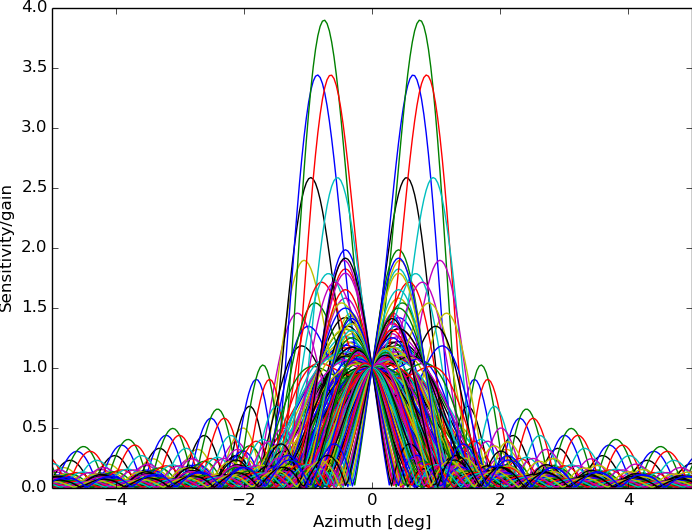
\includegraphics[width=0.49\linewidth]{gfx/4_window_response.png}}\hfill
\subfloat[Mean images]{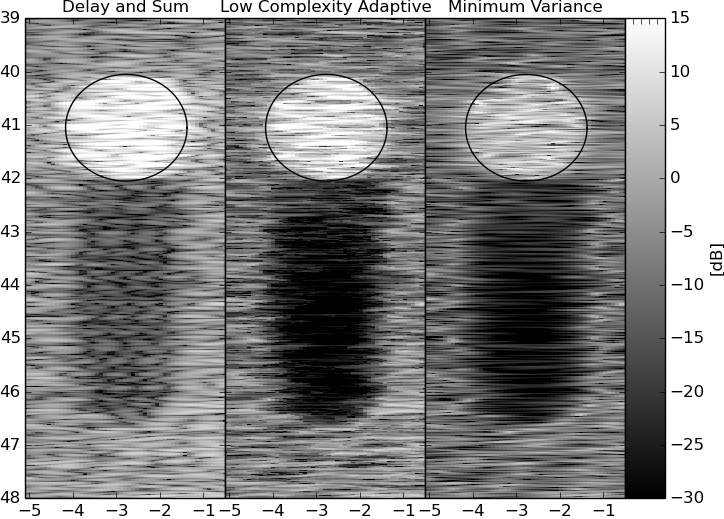
\includegraphics[width=0.49\linewidth]{gfx/4_mean_imgs.png}}\\
\subfloat[Windows ($\beta$)]{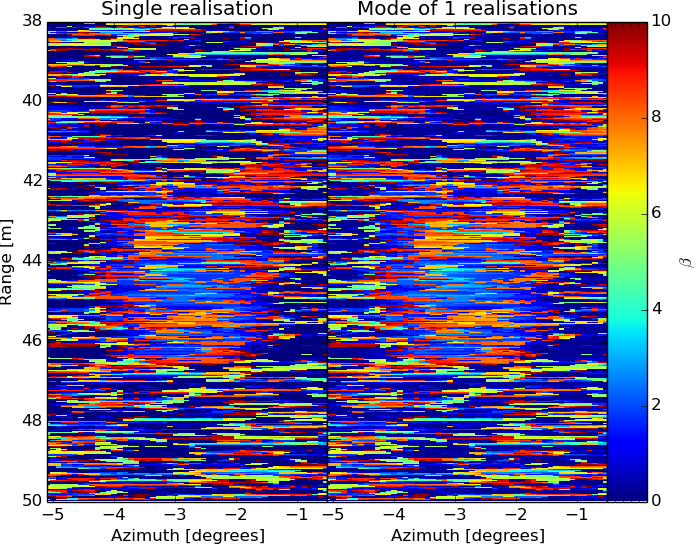
\includegraphics[width=0.49\linewidth]{gfx/4_windows_beta.png}}\hfill
\subfloat[Windows ($\phi$)]{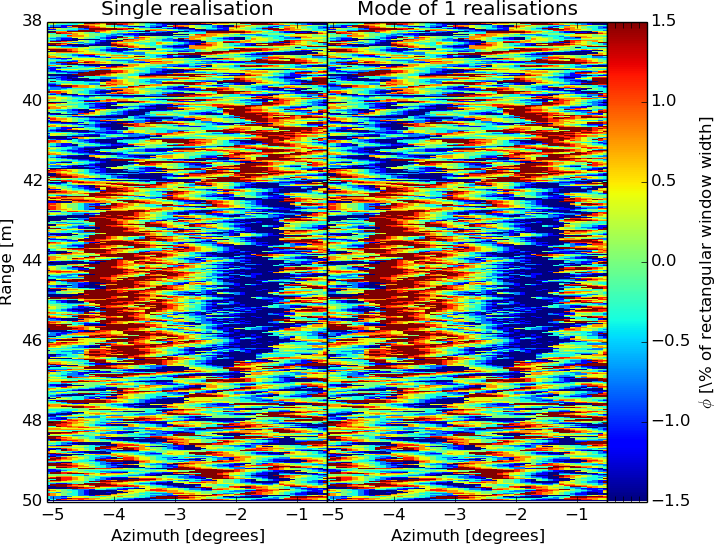
\includegraphics[width=0.48\linewidth]{gfx/4_windows_phi.png}}\\
\subfloat[Capon win. resp. through shadow]{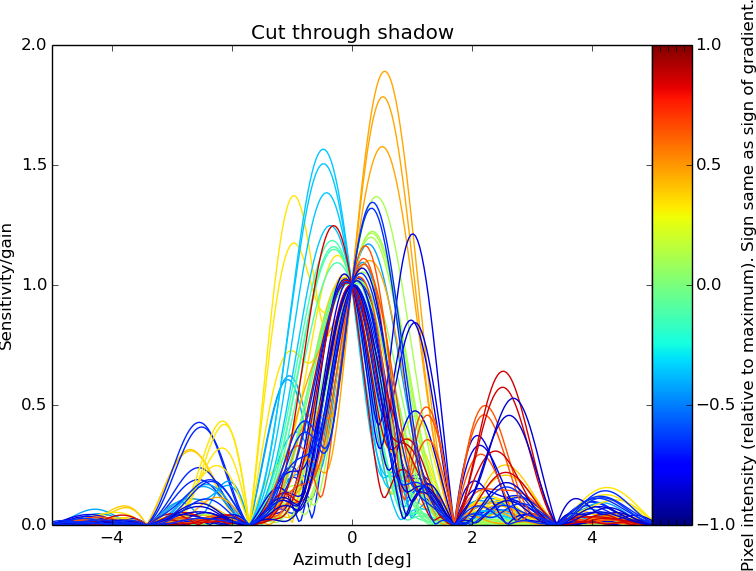
\includegraphics[width=0.49\linewidth]{gfx/4_win_resp_cut_shadow.png}}\hfill
\subfloat[Capon win. resp. through highlight]{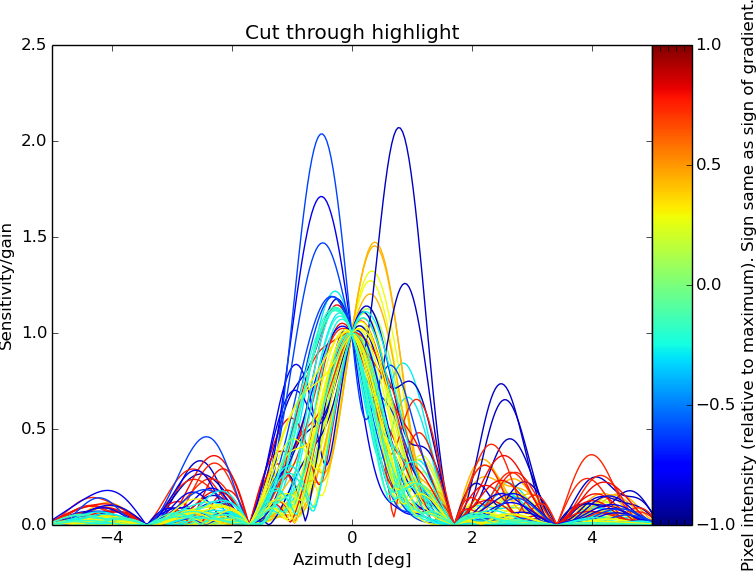
\includegraphics[width=0.49\linewidth]{gfx/4_win_resp_cut_highlight.png}}\\
\end{narrow}
\end{figure*}
\newpage
\begin{figure*}[!t]
\begin{narrow}{-1.2cm}{-1.2cm}\centering\vspace{-1.0cm}
\textbf{5. Capon: Tuning subarray.}\\
\begin{tabular}[c]{l l l l}
\bf General & M = 32                            & $\Delta r = \frac{c}{2B}$ = 2.5 cm & $\frac{640\,\text{pixels}] / 12\,\text{m}}{\Delta r} = \frac{4}{3}$ \\
\bf LCA     & $\beta \in [0,10]$ (9 values) & $\phi \in [-1.07,1.07]$ deg (9 values) & Navg = 3 \\
\bf Capon   & $\Delta$ = 0.01                 & L = 16                           & Navg = 3 \\
\end{tabular}
\subfloat[LCA Window Response]{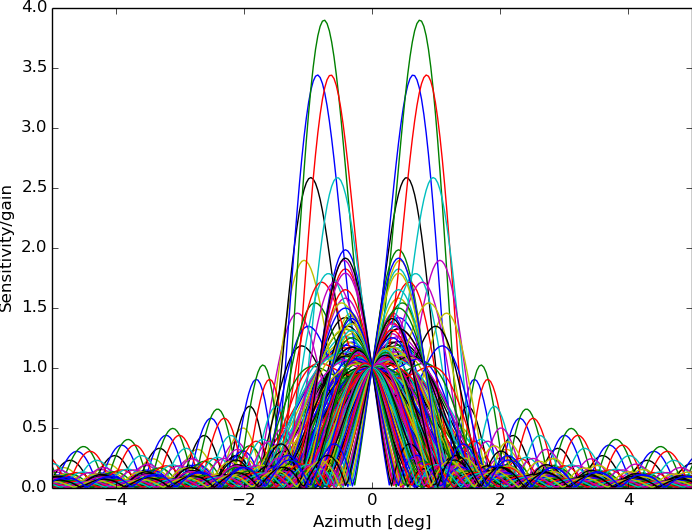
\includegraphics[width=0.49\linewidth]{gfx/5_window_response.png}}\hfill
\subfloat[Mean images]{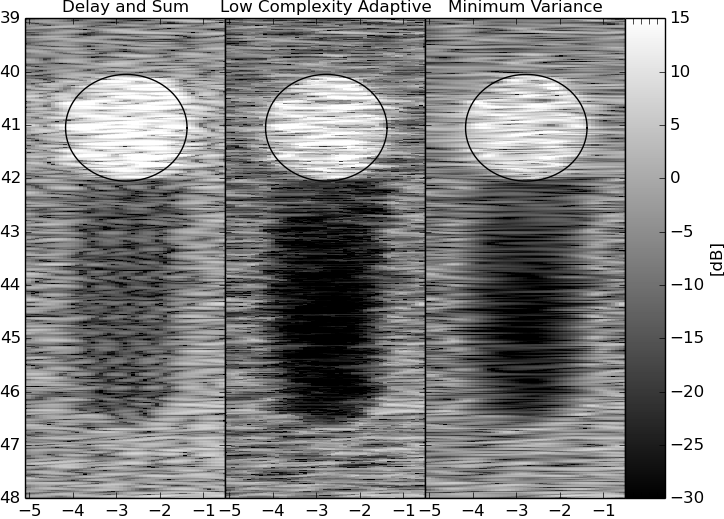
\includegraphics[width=0.49\linewidth]{gfx/5_mean_imgs.png}}\\
\subfloat[Windows ($\beta$)]{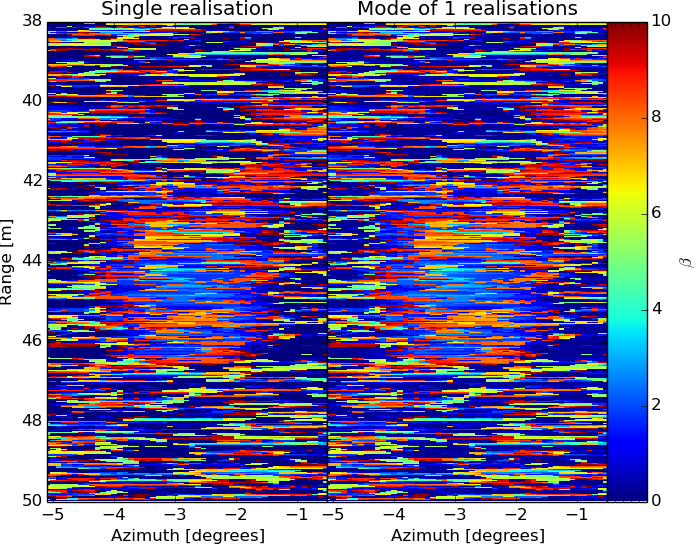
\includegraphics[width=0.49\linewidth]{gfx/5_windows_beta.png}}\hfill
\subfloat[Windows ($\phi$)]{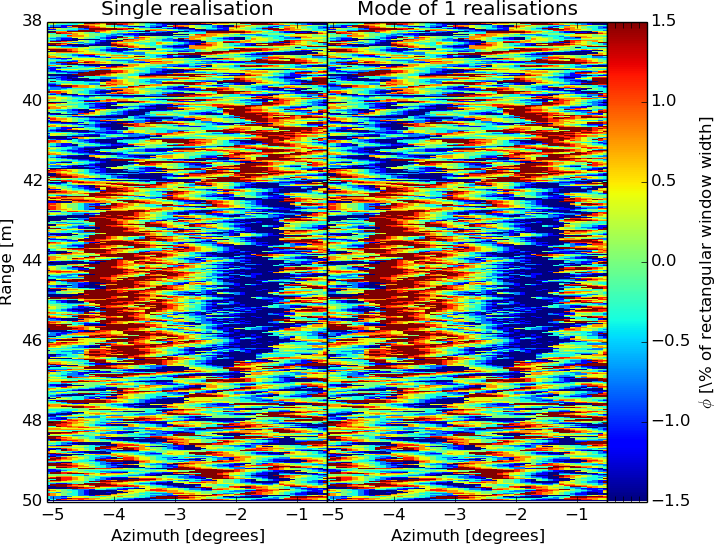
\includegraphics[width=0.48\linewidth]{gfx/5_windows_phi.png}}\\
\subfloat[Capon win. resp. through shadow]{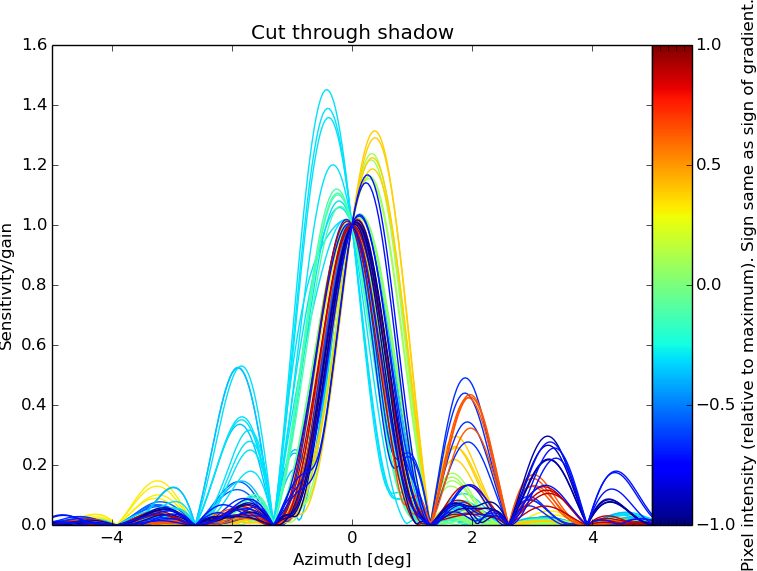
\includegraphics[width=0.49\linewidth]{gfx/5_win_resp_cut_shadow.png}}\hfill
\subfloat[Capon win. resp. through highlight]{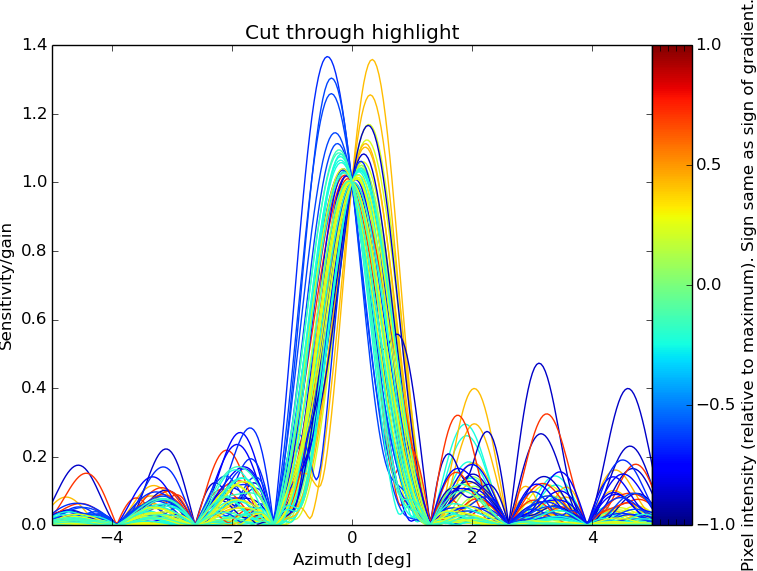
\includegraphics[width=0.49\linewidth]{gfx/5_win_resp_cut_highlight.png}}\\
\end{narrow}
\end{figure*}
\newpage
\begin{figure*}[!t]
\begin{narrow}{-1.2cm}{-1.2cm}\centering\vspace{-1.0cm}
\textbf{6. Capon: Tuning subarray.}\\
\begin{tabular}[c]{l l l l}
\bf General & M = 32                            & $\Delta r = \frac{c}{2B}$ = 2.5 cm & $\frac{640\,\text{pixels}] / 12\,\text{m}}{\Delta r} = \frac{4}{3}$ \\
\bf LCA     & $\beta \in [0,10]$ (9 values) & $\phi \in [-1.07,1.07]$ deg (9 values) & Navg = 3 \\
\bf Capon   & $\Delta$ = 0.01                 & L = 12                           & Navg = 3 \\
\end{tabular}
\subfloat[LCA Window Response]{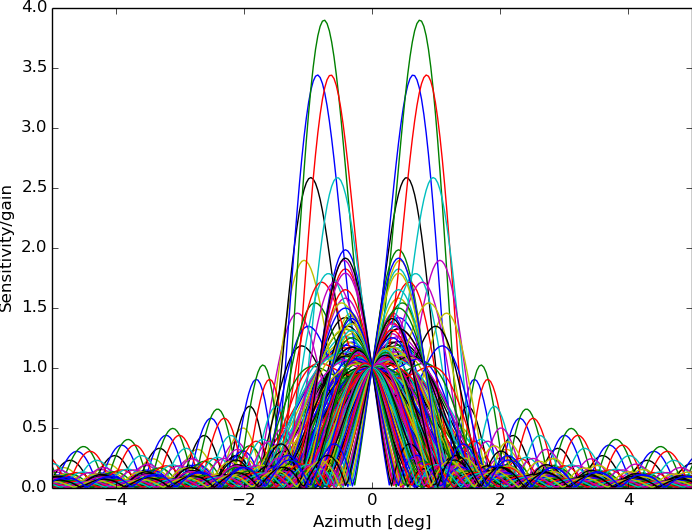
\includegraphics[width=0.49\linewidth]{gfx/6_window_response.png}}\hfill
\subfloat[Mean images]{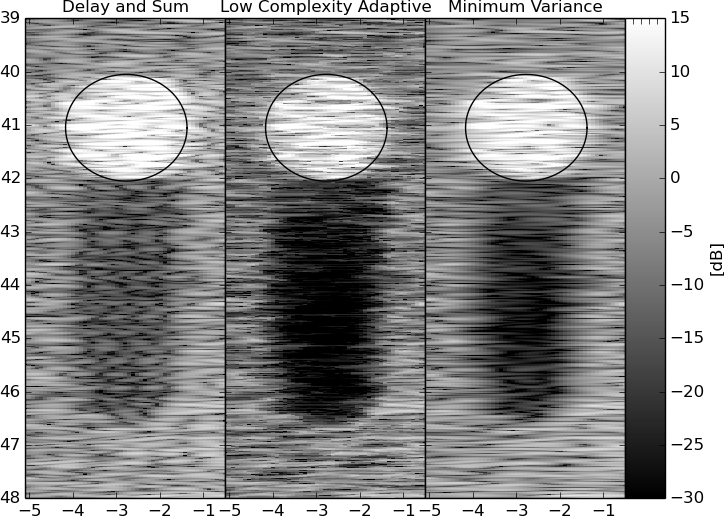
\includegraphics[width=0.49\linewidth]{gfx/6_mean_imgs.png}}\\
\subfloat[Windows ($\beta$)]{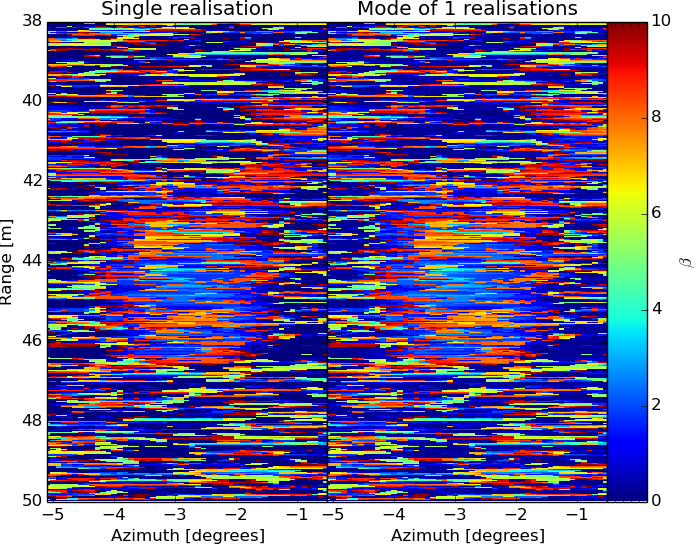
\includegraphics[width=0.49\linewidth]{gfx/6_windows_beta.png}}\hfill
\subfloat[Windows ($\phi$)]{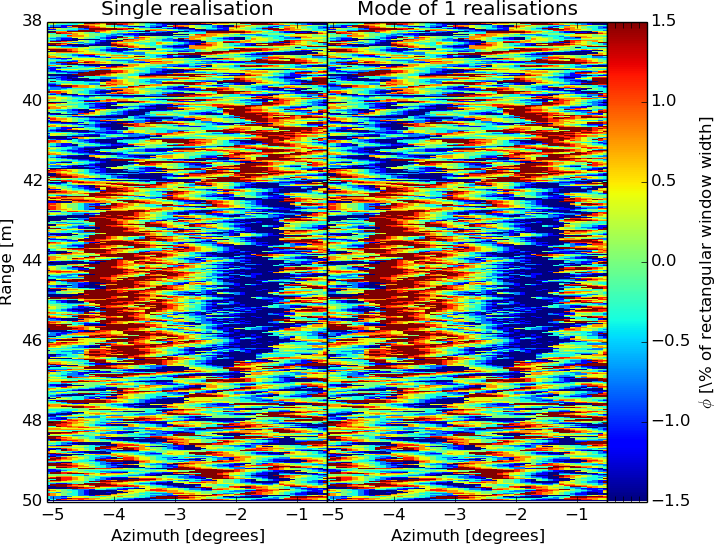
\includegraphics[width=0.48\linewidth]{gfx/6_windows_phi.png}}\\
\subfloat[Capon win. resp. through shadow]{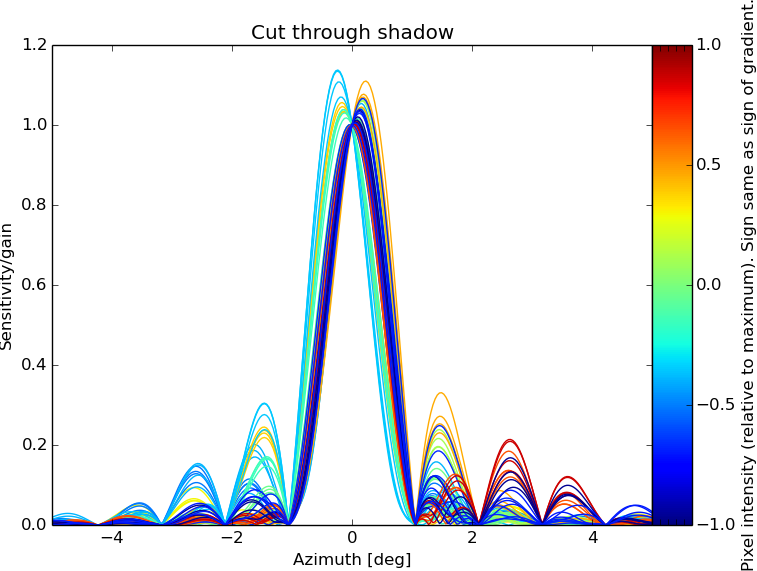
\includegraphics[width=0.49\linewidth]{gfx/6_win_resp_cut_shadow.png}}\hfill
\subfloat[Capon win. resp. through highlight]{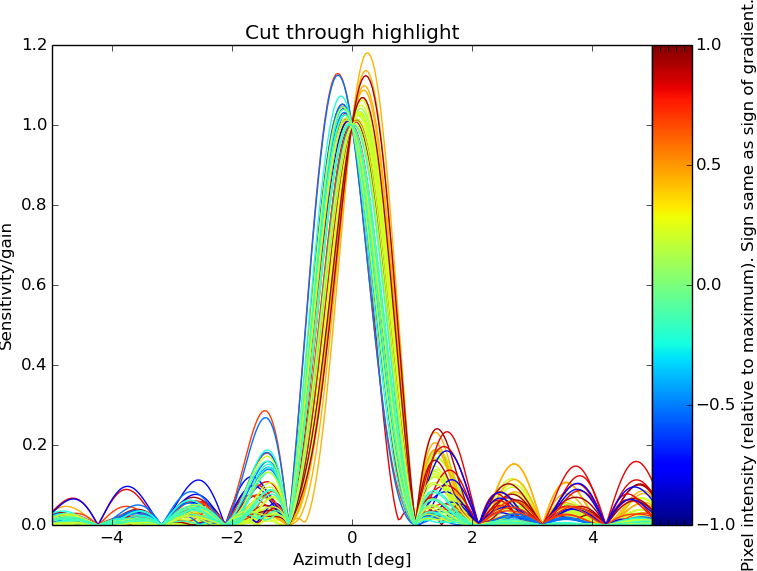
\includegraphics[width=0.49\linewidth]{gfx/6_win_resp_cut_highlight.png}}\\
\end{narrow}
\end{figure*}
\newpage
\begin{figure*}[!t]
\begin{narrow}{-1.2cm}{-1.2cm}\centering\vspace{-1.0cm}
\textbf{7. Capon: Tuning time averaging.}\\
\begin{tabular}[c]{l l l l}
\bf General & M = 32                            & $\Delta r = \frac{c}{2B}$ = 2.5 cm & $\frac{640\,\text{pixels}] / 12\,\text{m}}{\Delta r} = \frac{4}{3}$ \\
\bf LCA     & $\beta \in [0,10]$ (9 values) & $\phi \in [-1.07,1.07]$ deg (9 values) & Navg = 1 \\
\bf Capon   & $\Delta$ = 0.01                 & L = 16                           & Navg = 1 \\
\end{tabular}
\subfloat[LCA Window Response]{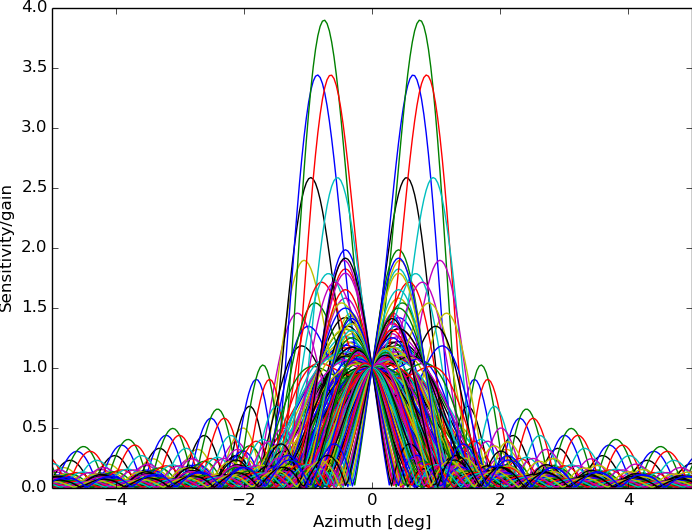
\includegraphics[width=0.49\linewidth]{gfx/7_window_response.png}}\hfill
\subfloat[Mean images]{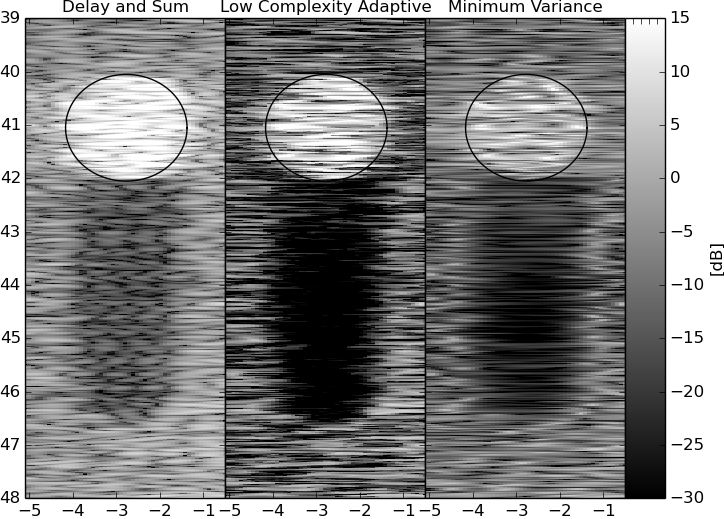
\includegraphics[width=0.49\linewidth]{gfx/7_mean_imgs.png}}\\
\subfloat[Windows ($\beta$)]{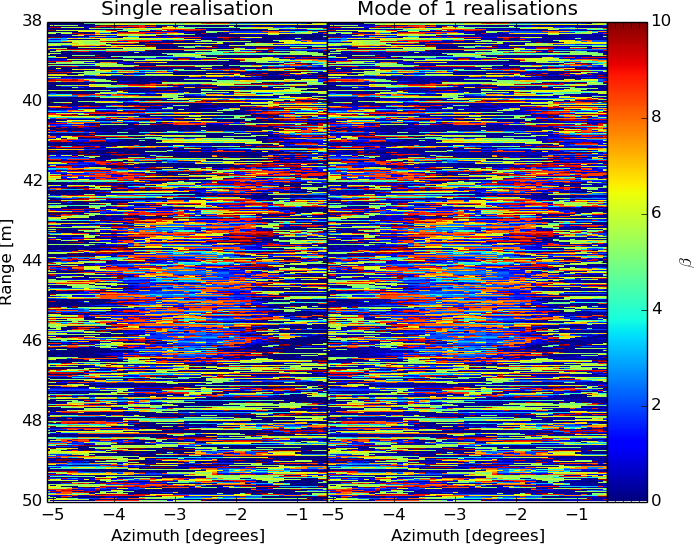
\includegraphics[width=0.49\linewidth]{gfx/7_windows_beta.png}}\hfill
\subfloat[Windows ($\phi$)]{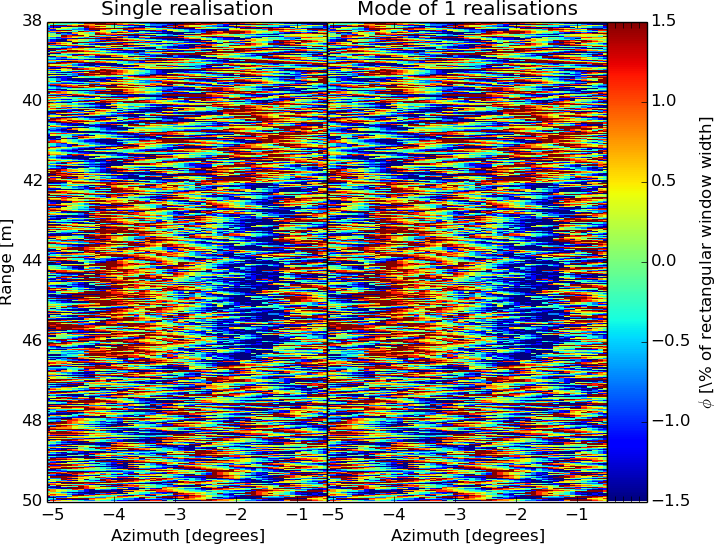
\includegraphics[width=0.48\linewidth]{gfx/7_windows_phi.png}}\\
\subfloat[Capon win. resp. through shadow]{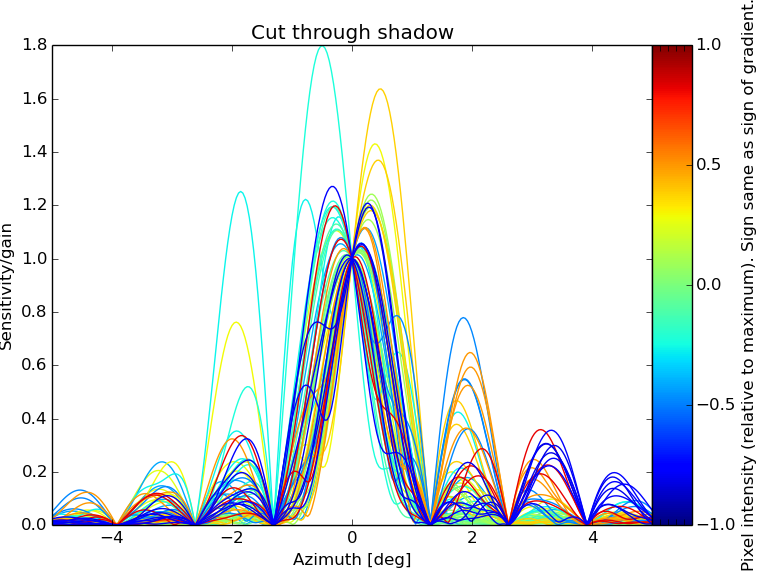
\includegraphics[width=0.49\linewidth]{gfx/7_win_resp_cut_shadow.png}}\hfill
\subfloat[Capon win. resp. through highlight]{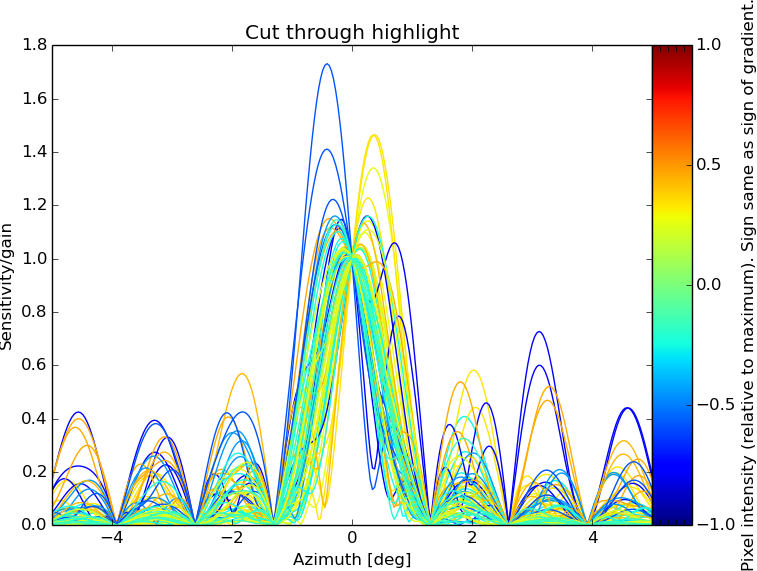
\includegraphics[width=0.49\linewidth]{gfx/7_win_resp_cut_highlight.png}}\\
\end{narrow}
\end{figure*}
\newpage
\begin{figure*}[!t]
\begin{narrow}{-1.2cm}{-1.2cm}\centering\vspace{-1.0cm}
\textbf{8. Capon: Tuning time averaging.}\\
\begin{tabular}[c]{l l l l}
\bf General & M = 32                            & $\Delta r = \frac{c}{2B}$ = 2.5 cm & $\frac{640\,\text{pixels}] / 12\,\text{m}}{\Delta r} = \frac{4}{3}$ \\
\bf LCA     & $\beta \in [0,10]$ (9 values) & $\phi \in [-1.07,1.07]$ deg (9 values) & Navg = 3 \\
\bf Capon   & $\Delta$ = 0.01                 & L = 16                           & Navg = 3 \\
\end{tabular}
\subfloat[LCA Window Response]{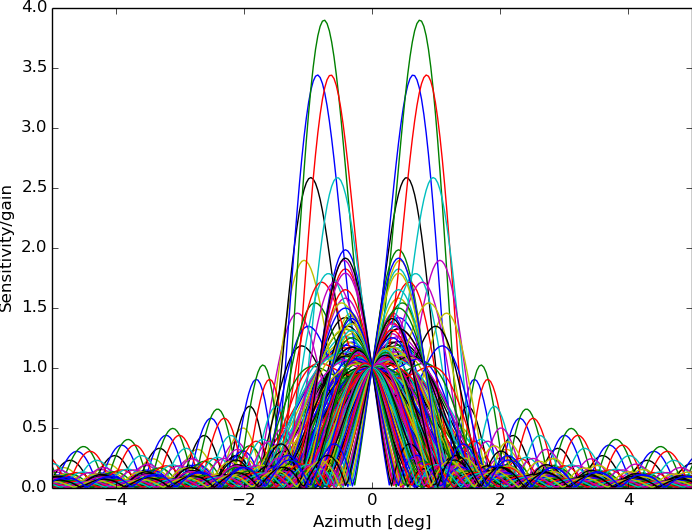
\includegraphics[width=0.49\linewidth]{gfx/8_window_response.png}}\hfill
\subfloat[Mean images]{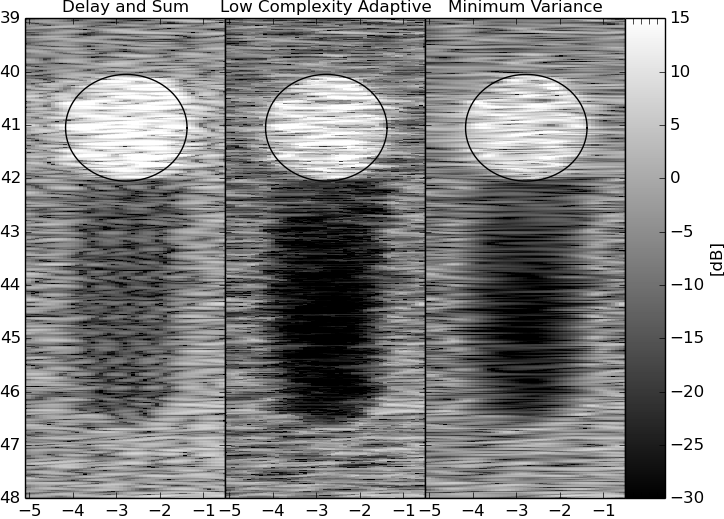
\includegraphics[width=0.49\linewidth]{gfx/8_mean_imgs.png}}\\
\subfloat[Windows ($\beta$)]{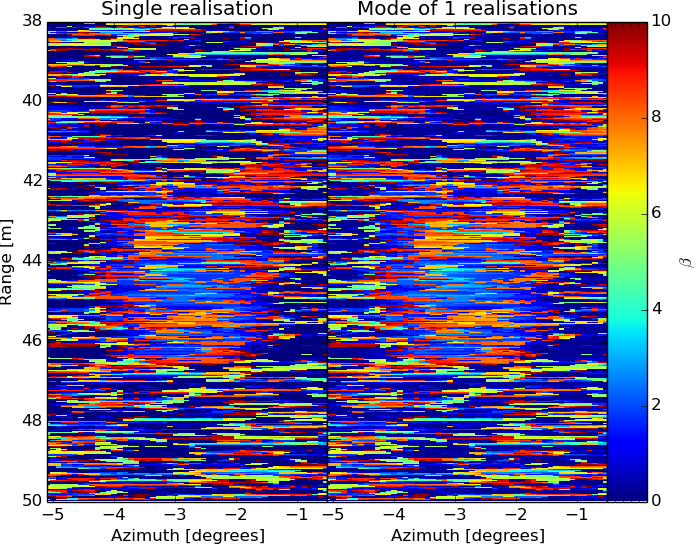
\includegraphics[width=0.49\linewidth]{gfx/8_windows_beta.png}}\hfill
\subfloat[Windows ($\phi$)]{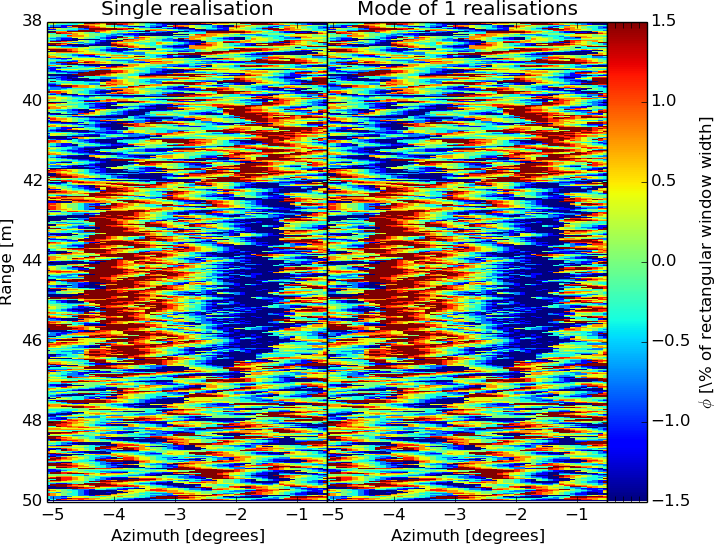
\includegraphics[width=0.48\linewidth]{gfx/8_windows_phi.png}}\\
\subfloat[Capon win. resp. through shadow]{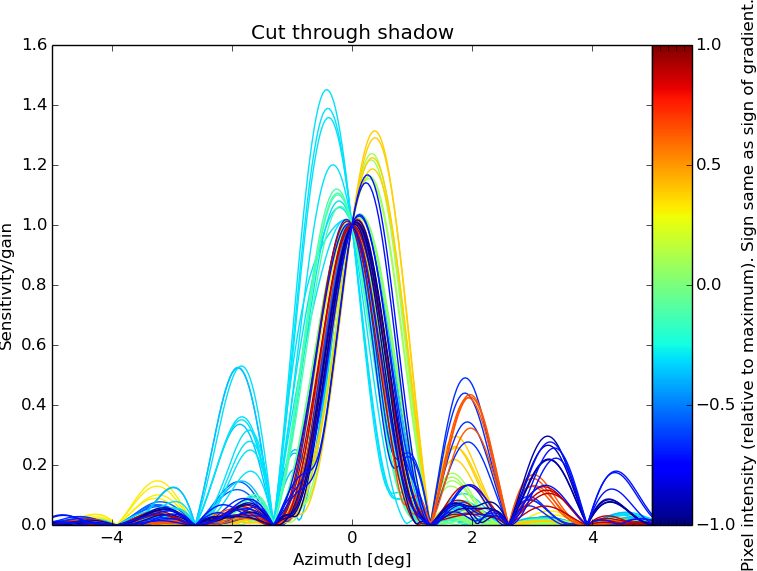
\includegraphics[width=0.49\linewidth]{gfx/8_win_resp_cut_shadow.png}}\hfill
\subfloat[Capon win. resp. through highlight]{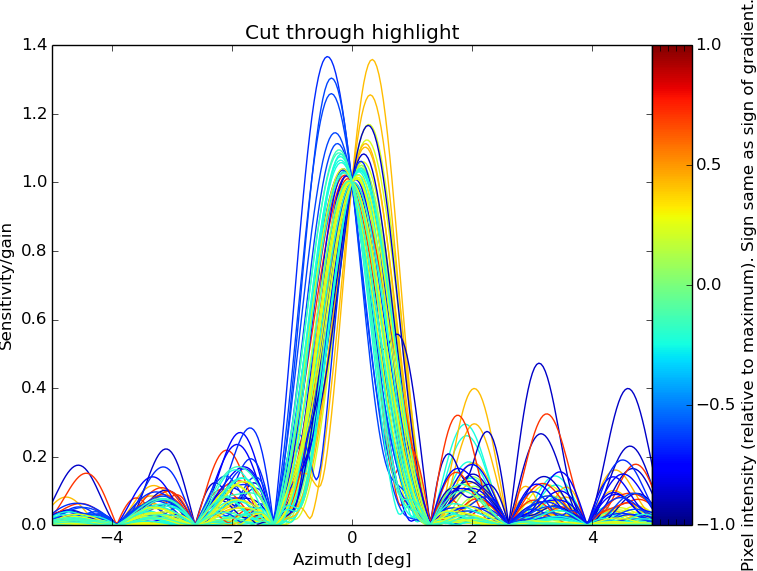
\includegraphics[width=0.49\linewidth]{gfx/8_win_resp_cut_highlight.png}}\\
\end{narrow}
\end{figure*}
\newpage
\begin{figure*}[!t]
\begin{narrow}{-1.2cm}{-1.2cm}\centering\vspace{-1.0cm}
\textbf{9. Capon: Tuning time averaging.}\\
\begin{tabular}[c]{l l l l}
\bf General & M = 32                            & $\Delta r = \frac{c}{2B}$ = 2.5 cm & $\frac{640\,\text{pixels}] / 12\,\text{m}}{\Delta r} = \frac{4}{3}$ \\
\bf LCA     & $\beta \in [0,10]$ (9 values) & $\phi \in [-1.07,1.07]$ deg (9 values) & Navg = 5 \\
\bf Capon   & $\Delta$ = 0.01                 & L = 16                           & Navg = 5 \\
\end{tabular}
\subfloat[LCA Window Response]{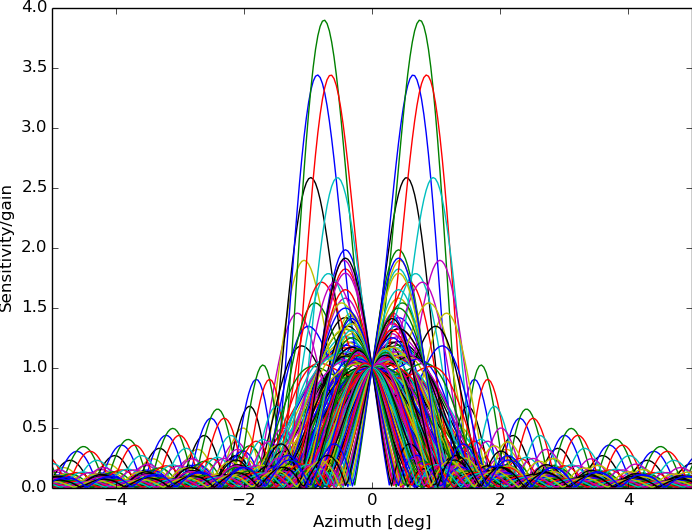
\includegraphics[width=0.49\linewidth]{gfx/9_window_response.png}}\hfill
\subfloat[Mean images]{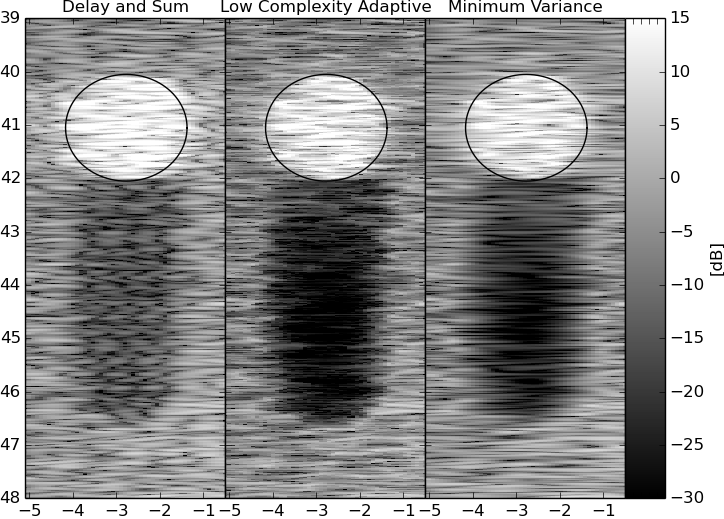
\includegraphics[width=0.49\linewidth]{gfx/9_mean_imgs.png}}\\
\subfloat[Windows ($\beta$)]{\includegraphics[width=0.49\linewidth]{gfx/9_windows_beta.png}}\hfill
\subfloat[Windows ($\phi$)]{\includegraphics[width=0.48\linewidth]{gfx/9_windows_phi.png}}\\
\subfloat[Capon win. resp. through shadow]{\includegraphics[width=0.49\linewidth]{gfx/9_win_resp_cut_shadow.png}}\hfill
\subfloat[Capon win. resp. through highlight]{\includegraphics[width=0.49\linewidth]{gfx/9_win_resp_cut_highlight.png}}\\
\end{narrow}
\end{figure*}
\newpage
\begin{figure*}[!t]
\begin{narrow}{-1.2cm}{-1.2cm}\centering\vspace{-1.0cm}
\textbf{10. Capon: Tuning time averaging.}\\
\begin{tabular}[c]{l l l l}
\bf General & M = 32                            & $\Delta r = \frac{c}{2B}$ = 2.5 cm & $\frac{640\,\text{pixels}] / 12\,\text{m}}{\Delta r} = \frac{4}{3}$ \\
\bf LCA     & $\beta \in [0,10]$ (9 values) & $\phi \in [-1.07,1.07]$ deg (9 values) & Navg = 7 \\
\bf Capon   & $\Delta$ = 0.01                 & L = 16                           & Navg = 7 \\
\end{tabular}
\subfloat[LCA Window Response]{\includegraphics[width=0.49\linewidth]{gfx/10_window_response.png}}\hfill
\subfloat[Mean images]{\includegraphics[width=0.49\linewidth]{gfx/10_mean_imgs.png}}\\
\subfloat[Windows ($\beta$)]{\includegraphics[width=0.49\linewidth]{gfx/10_windows_beta.png}}\hfill
\subfloat[Windows ($\phi$)]{\includegraphics[width=0.48\linewidth]{gfx/10_windows_phi.png}}\\
\subfloat[Capon win. resp. through shadow]{\includegraphics[width=0.49\linewidth]{gfx/10_win_resp_cut_shadow.png}}\hfill
\subfloat[Capon win. resp. through highlight]{\includegraphics[width=0.49\linewidth]{gfx/10_win_resp_cut_highlight.png}}\\
\end{narrow}
\end{figure*}
\newpage
\begin{figure*}[!t]
\begin{narrow}{-1.2cm}{-1.2cm}\centering\vspace{-1.0cm}
\textbf{11. LCA: Reasonable settings.}\\
\begin{tabular}[c]{l l l l}
\bf General & M = 32                            & $\Delta r = \frac{c}{2B}$ = 2.5 cm & $\frac{640\,\text{pixels}] / 12\,\text{m}}{\Delta r} = \frac{4}{3}$ \\
\bf LCA     & $\beta \in [0,10]$ (9 values) & $\phi \in [-0.57,0.57]$ deg (9 values) & Navg = 7 \\
\bf Capon   & $\Delta$ = 0.01                 & L = 16                           & Navg = 7 \\
\end{tabular}
\subfloat[LCA Window Response]{\includegraphics[width=0.49\linewidth]{gfx/11_window_response.png}}\hfill
\subfloat[Mean images]{\includegraphics[width=0.49\linewidth]{gfx/11_mean_imgs.png}}\\
\subfloat[Windows ($\beta$)]{\includegraphics[width=0.49\linewidth]{gfx/11_windows_beta.png}}\hfill
\subfloat[Windows ($\phi$)]{\includegraphics[width=0.48\linewidth]{gfx/11_windows_phi.png}}\\
\subfloat[Capon win. resp. through shadow]{\includegraphics[width=0.49\linewidth]{gfx/11_win_resp_cut_shadow.png}}\hfill
\subfloat[Capon win. resp. through highlight]{\includegraphics[width=0.49\linewidth]{gfx/11_win_resp_cut_highlight.png}}\\
\end{narrow}
\end{figure*}
\newpage
\begin{figure*}[!t]
\begin{narrow}{-1.2cm}{-1.2cm}\centering\vspace{-1.0cm}
\textbf{12. LCA: Lots of Kaiser windows - wide span.}\\
\begin{tabular}[c]{l l l l}
\bf General & M = 32                            & $\Delta r = \frac{c}{2B}$ = 2.5 cm & $\frac{640\,\text{pixels}] / 12\,\text{m}}{\Delta r} = \frac{4}{3}$ \\
\bf LCA     & $\beta \in [0,20]$ (19 values) & $\phi \in [-1.07,1.07]$ deg (19 values) & Navg = 7 \\
\bf Capon   & $\Delta$ = 0.01                 & L = 16                           & Navg = 7 \\
\end{tabular}
\subfloat[LCA Window Response]{\includegraphics[width=0.49\linewidth]{gfx/12_window_response.png}}\hfill
\subfloat[Mean images]{\includegraphics[width=0.49\linewidth]{gfx/12_mean_imgs.png}}\\
\subfloat[Windows ($\beta$)]{\includegraphics[width=0.49\linewidth]{gfx/12_windows_beta.png}}\hfill
\subfloat[Windows ($\phi$)]{\includegraphics[width=0.48\linewidth]{gfx/12_windows_phi.png}}\\
\subfloat[Capon win. resp. through shadow]{\includegraphics[width=0.49\linewidth]{gfx/12_win_resp_cut_shadow.png}}\hfill
\subfloat[Capon win. resp. through highlight]{\includegraphics[width=0.49\linewidth]{gfx/12_win_resp_cut_highlight.png}}\\
\end{narrow}
\end{figure*}
\newpage
\begin{figure*}[!t]
\begin{narrow}{-1.2cm}{-1.2cm}\centering\vspace{-1.0cm}
\textbf{13. LCA: Lots of trigonometric windows - wide span.}\\
\begin{tabular}[c]{l l l l}
\bf General & M = 32                            & $\Delta r = \frac{c}{2B}$ = 2.5 cm & $\frac{640\,\text{pixels}] / 12\,\text{m}}{\Delta r} = \frac{4}{3}$ \\
\bf LCA     & $\beta \in [0,20]$ (19 values) & $\phi \in [-1.07,1.07]$ deg (19 values) & Navg = 7 \\
\bf Capon   & $\Delta$ = 0.01                 & L = 16                           & Navg = 7 \\
\end{tabular}
\subfloat[LCA Window Response]{\includegraphics[width=0.49\linewidth]{gfx/13_window_response.png}}\hfill
\subfloat[Mean images]{\includegraphics[width=0.49\linewidth]{gfx/13_mean_imgs.png}}\\
\subfloat[Windows ($\beta$)]{\includegraphics[width=0.49\linewidth]{gfx/13_windows_beta.png}}\hfill
\subfloat[Windows ($\phi$)]{\includegraphics[width=0.48\linewidth]{gfx/13_windows_phi.png}}\\
\subfloat[Capon win. resp. through shadow]{\includegraphics[width=0.49\linewidth]{gfx/13_win_resp_cut_shadow.png}}\hfill
\subfloat[Capon win. resp. through highlight]{\includegraphics[width=0.49\linewidth]{gfx/13_win_resp_cut_highlight.png}}\\
\end{narrow}
\end{figure*}
\newpage
\begin{figure*}[!t]
\begin{narrow}{-1.2cm}{-1.2cm}\centering\vspace{-1.0cm}
\textbf{14. LCA: Back on Kaiser - reducing steering span.}\\
\begin{tabular}[c]{l l l l}
\bf General & M = 32                            & $\Delta r = \frac{c}{2B}$ = 2.5 cm & $\frac{640\,\text{pixels}] / 12\,\text{m}}{\Delta r} = \frac{4}{3}$ \\
\bf LCA     & $\beta \in [0,20]$ (19 values) & $\phi \in [-0.72,0.72]$ deg (19 values) & Navg = 7 \\
\bf Capon   & $\Delta$ = 0.01                 & L = 16                           & Navg = 7 \\
\end{tabular}
\subfloat[LCA Window Response]{\includegraphics[width=0.49\linewidth]{gfx/14_window_response.png}}\hfill
\subfloat[Mean images]{\includegraphics[width=0.49\linewidth]{gfx/14_mean_imgs.png}}\\
\subfloat[Windows ($\beta$)]{\includegraphics[width=0.49\linewidth]{gfx/14_windows_beta.png}}\hfill
\subfloat[Windows ($\phi$)]{\includegraphics[width=0.48\linewidth]{gfx/14_windows_phi.png}}\\
\subfloat[Capon win. resp. through shadow]{\includegraphics[width=0.49\linewidth]{gfx/14_win_resp_cut_shadow.png}}\hfill
\subfloat[Capon win. resp. through highlight]{\includegraphics[width=0.49\linewidth]{gfx/14_win_resp_cut_highlight.png}}\\
\end{narrow}
\end{figure*}
\newpage
\begin{figure*}[!t]
\begin{narrow}{-1.2cm}{-1.2cm}\centering\vspace{-1.0cm}
\textbf{15. LCA: Reducing steering span.}\\
\begin{tabular}[c]{l l l l}
\bf General & M = 32                            & $\Delta r = \frac{c}{2B}$ = 2.5 cm & $\frac{640\,\text{pixels}] / 12\,\text{m}}{\Delta r} = \frac{4}{3}$ \\
\bf LCA     & $\beta \in [0,20]$ (19 values) & $\phi \in [-0.36,0.36]$ deg (19 values) & Navg = 7 \\
\bf Capon   & $\Delta$ = 0.01                 & L = 16                           & Navg = 7 \\
\end{tabular}
\subfloat[LCA Window Response]{\includegraphics[width=0.49\linewidth]{gfx/15_window_response.png}}\hfill
\subfloat[Mean images]{\includegraphics[width=0.49\linewidth]{gfx/15_mean_imgs.png}}\\
\subfloat[Windows ($\beta$)]{\includegraphics[width=0.49\linewidth]{gfx/15_windows_beta.png}}\hfill
\subfloat[Windows ($\phi$)]{\includegraphics[width=0.48\linewidth]{gfx/15_windows_phi.png}}\\
\subfloat[Capon win. resp. through shadow]{\includegraphics[width=0.49\linewidth]{gfx/15_win_resp_cut_shadow.png}}\hfill
\subfloat[Capon win. resp. through highlight]{\includegraphics[width=0.49\linewidth]{gfx/15_win_resp_cut_highlight.png}}\\
\end{narrow}
\end{figure*}
\newpage
\begin{figure*}[!t]
\begin{narrow}{-1.2cm}{-1.2cm}\centering\vspace{-1.0cm}
\textbf{16. LCA: Adjusting resolution/SNR.}\\
\begin{tabular}[c]{l l l l}
\bf General & M = 32                            & $\Delta r = \frac{c}{2B}$ = 2.5 cm & $\frac{640\,\text{pixels}] / 12\,\text{m}}{\Delta r} = \frac{4}{3}$ \\
\bf LCA     & $\beta \in [0,5]$ (19 values) & $\phi \in [-0.72,0.72]$ deg (19 values) & Navg = 7 \\
\bf Capon   & $\Delta$ = 0.01                 & L = 16                           & Navg = 7 \\
\end{tabular}
\subfloat[LCA Window Response]{\includegraphics[width=0.49\linewidth]{gfx/16_window_response.png}}\hfill
\subfloat[Mean images]{\includegraphics[width=0.49\linewidth]{gfx/16_mean_imgs.png}}\\
\subfloat[Windows ($\beta$)]{\includegraphics[width=0.49\linewidth]{gfx/16_windows_beta.png}}\hfill
\subfloat[Windows ($\phi$)]{\includegraphics[width=0.48\linewidth]{gfx/16_windows_phi.png}}\\
\subfloat[Capon win. resp. through shadow]{\includegraphics[width=0.49\linewidth]{gfx/16_win_resp_cut_shadow.png}}\hfill
\subfloat[Capon win. resp. through highlight]{\includegraphics[width=0.49\linewidth]{gfx/16_win_resp_cut_highlight.png}}\\
\end{narrow}
\end{figure*}
\newpage
\begin{figure*}[!t]
\begin{narrow}{-1.2cm}{-1.2cm}\centering\vspace{-1.0cm}
\textbf{17. LCA: Adjusting resolution/SNR.}\\
\begin{tabular}[c]{l l l l}
\bf General & M = 32                            & $\Delta r = \frac{c}{2B}$ = 2.5 cm & $\frac{640\,\text{pixels}] / 12\,\text{m}}{\Delta r} = \frac{4}{3}$ \\
\bf LCA     & $\beta \in [5,20]$ (19 values) & $\phi \in [-0.72,0.72]$ deg (19 values) & Navg = 7 \\
\bf Capon   & $\Delta$ = 0.01                 & L = 16                           & Navg = 7 \\
\end{tabular}
\subfloat[LCA Window Response]{\includegraphics[width=0.49\linewidth]{gfx/17_window_response.png}}\hfill
\subfloat[Mean images]{\includegraphics[width=0.49\linewidth]{gfx/17_mean_imgs.png}}\\
\subfloat[Windows ($\beta$)]{\includegraphics[width=0.49\linewidth]{gfx/17_windows_beta.png}}\hfill
\subfloat[Windows ($\phi$)]{\includegraphics[width=0.48\linewidth]{gfx/17_windows_phi.png}}\\
\subfloat[Capon win. resp. through shadow]{\includegraphics[width=0.49\linewidth]{gfx/17_win_resp_cut_shadow.png}}\hfill
\subfloat[Capon win. resp. through highlight]{\includegraphics[width=0.49\linewidth]{gfx/17_win_resp_cut_highlight.png}}\\
\end{narrow}
\end{figure*}
\newpage
\begin{figure*}[!t]
\begin{narrow}{-1.2cm}{-1.2cm}\centering\vspace{-1.0cm}
\textbf{18. LCA: Fewer windows.}\\
\begin{tabular}[c]{l l l l}
\bf General & M = 32                            & $\Delta r = \frac{c}{2B}$ = 2.5 cm & $\frac{640\,\text{pixels}] / 12\,\text{m}}{\Delta r} = \frac{4}{3}$ \\
\bf LCA     & $\beta \in [0,10]$ (9 values) & $\phi \in [-0.72,0.72]$ deg (19 values) & Navg = 7 \\
\bf Capon   & $\Delta$ = 0.01                 & L = 16                           & Navg = 7 \\
\end{tabular}
\subfloat[LCA Window Response]{\includegraphics[width=0.49\linewidth]{gfx/18_window_response.png}}\hfill
\subfloat[Mean images]{\includegraphics[width=0.49\linewidth]{gfx/18_mean_imgs.png}}\\
\subfloat[Windows ($\beta$)]{\includegraphics[width=0.49\linewidth]{gfx/18_windows_beta.png}}\hfill
\subfloat[Windows ($\phi$)]{\includegraphics[width=0.48\linewidth]{gfx/18_windows_phi.png}}\\
\subfloat[Capon win. resp. through shadow]{\includegraphics[width=0.49\linewidth]{gfx/18_win_resp_cut_shadow.png}}\hfill
\subfloat[Capon win. resp. through highlight]{\includegraphics[width=0.49\linewidth]{gfx/18_win_resp_cut_highlight.png}}\\
\end{narrow}
\end{figure*}
\newpage
\begin{figure*}[!t]
\begin{narrow}{-1.2cm}{-1.2cm}\centering\vspace{-1.0cm}
\textbf{19. LCA: Fewer steering angles.}\\
\begin{tabular}[c]{l l l l}
\bf General & M = 32                            & $\Delta r = \frac{c}{2B}$ = 2.5 cm & $\frac{640\,\text{pixels}] / 12\,\text{m}}{\Delta r} = \frac{4}{3}$ \\
\bf LCA     & $\beta \in [0,10]$ (19 values) & $\phi \in [-0.72,0.72]$ deg (9 values) & Navg = 7 \\
\bf Capon   & $\Delta$ = 0.01                 & L = 16                           & Navg = 7 \\
\end{tabular}
\subfloat[LCA Window Response]{\includegraphics[width=0.49\linewidth]{gfx/19_window_response.png}}\hfill
\subfloat[Mean images]{\includegraphics[width=0.49\linewidth]{gfx/19_mean_imgs.png}}\\
\subfloat[Windows ($\beta$)]{\includegraphics[width=0.49\linewidth]{gfx/19_windows_beta.png}}\hfill
\subfloat[Windows ($\phi$)]{\includegraphics[width=0.48\linewidth]{gfx/19_windows_phi.png}}\\
\subfloat[Capon win. resp. through shadow]{\includegraphics[width=0.49\linewidth]{gfx/19_win_resp_cut_shadow.png}}\hfill
\subfloat[Capon win. resp. through highlight]{\includegraphics[width=0.49\linewidth]{gfx/19_win_resp_cut_highlight.png}}\\
\end{narrow}
\end{figure*}
\newpage
\begin{figure*}[!t]
\begin{narrow}{-1.2cm}{-1.2cm}\centering\vspace{-1.0cm}
\textbf{20. LCA: Fewer both.}\\
\begin{tabular}[c]{l l l l}
\bf General & M = 32                            & $\Delta r = \frac{c}{2B}$ = 2.5 cm & $\frac{640\,\text{pixels}] / 12\,\text{m}}{\Delta r} = \frac{4}{3}$ \\
\bf LCA     & $\beta \in [0,10]$ (9 values) & $\phi \in [-0.72,0.72]$ deg (9 values) & Navg = 7 \\
\bf Capon   & $\Delta$ = 0.01                 & L = 16                           & Navg = 7 \\
\end{tabular}
\subfloat[LCA Window Response]{\includegraphics[width=0.49\linewidth]{gfx/20_window_response.png}}\hfill
\subfloat[Mean images]{\includegraphics[width=0.49\linewidth]{gfx/20_mean_imgs.png}}\\
\subfloat[Windows ($\beta$)]{\includegraphics[width=0.49\linewidth]{gfx/20_windows_beta.png}}\hfill
\subfloat[Windows ($\phi$)]{\includegraphics[width=0.48\linewidth]{gfx/20_windows_phi.png}}\\
\subfloat[Capon win. resp. through shadow]{\includegraphics[width=0.49\linewidth]{gfx/20_win_resp_cut_shadow.png}}\hfill
\subfloat[Capon win. resp. through highlight]{\includegraphics[width=0.49\linewidth]{gfx/20_win_resp_cut_highlight.png}}\\
\end{narrow}
\end{figure*}
\newpage
\begin{figure*}[!t]
\begin{narrow}{-1.2cm}{-1.2cm}\centering\vspace{-1.0cm}
\textbf{21. LCA: Even less.}\\
\begin{tabular}[c]{l l l l}
\bf General & M = 32                            & $\Delta r = \frac{c}{2B}$ = 2.5 cm & $\frac{640\,\text{pixels}] / 12\,\text{m}}{\Delta r} = \frac{4}{3}$ \\
\bf LCA     & $\beta \in [0,5]$ (9 values) & $\phi \in [-0.72,0.72]$ deg (5 values) & Navg = 7 \\
\bf Capon   & $\Delta$ = 0.01                 & L = 16                           & Navg = 7 \\
\end{tabular}
\subfloat[LCA Window Response]{\includegraphics[width=0.49\linewidth]{gfx/21_window_response.png}}\hfill
\subfloat[Mean images]{\includegraphics[width=0.49\linewidth]{gfx/21_mean_imgs.png}}\\
\subfloat[Windows ($\beta$)]{\includegraphics[width=0.49\linewidth]{gfx/21_windows_beta.png}}\hfill
\subfloat[Windows ($\phi$)]{\includegraphics[width=0.48\linewidth]{gfx/21_windows_phi.png}}\\
\subfloat[Capon win. resp. through shadow]{\includegraphics[width=0.49\linewidth]{gfx/21_win_resp_cut_shadow.png}}\hfill
\subfloat[Capon win. resp. through highlight]{\includegraphics[width=0.49\linewidth]{gfx/21_win_resp_cut_highlight.png}}\\
\end{narrow}
\end{figure*}
\newpage
\begin{figure*}[!t]
\begin{narrow}{-1.2cm}{-1.2cm}\centering\vspace{-1.0cm}
\textbf{22. LCA: Hardly any.}\\
\begin{tabular}[c]{l l l l}
\bf General & M = 32                            & $\Delta r = \frac{c}{2B}$ = 2.5 cm & $\frac{640\,\text{pixels}] / 12\,\text{m}}{\Delta r} = \frac{4}{3}$ \\
\bf LCA     & $\beta \in [0,5]$ (5 values) & $\phi \in [-0.72,0.72]$ deg (5 values) & Navg = 7 \\
\bf Capon   & $\Delta$ = 0.01                 & L = 16                           & Navg = 7 \\
\end{tabular}
\subfloat[LCA Window Response]{\includegraphics[width=0.49\linewidth]{gfx/22_window_response.png}}\hfill
\subfloat[Mean images]{\includegraphics[width=0.49\linewidth]{gfx/22_mean_imgs.png}}\\
\subfloat[Windows ($\beta$)]{\includegraphics[width=0.49\linewidth]{gfx/22_windows_beta.png}}\hfill
\subfloat[Windows ($\phi$)]{\includegraphics[width=0.48\linewidth]{gfx/22_windows_phi.png}}\\
\subfloat[Capon win. resp. through shadow]{\includegraphics[width=0.49\linewidth]{gfx/22_win_resp_cut_shadow.png}}\hfill
\subfloat[Capon win. resp. through highlight]{\includegraphics[width=0.49\linewidth]{gfx/22_win_resp_cut_highlight.png}}\\
\end{narrow}
\end{figure*}

% \begin{figure*}[!t]
% \centerline{\subfloat[Case I]\includegraphics[width=2.5in]{subfigcase1}%
% \label{fig_first_case}}
% \hfil
% \subfloat[Case II]{\includegraphics[width=2.5in]{subfigcase2}%
% \label{fig_second_case}}}
% \caption{Simulation results}
% \label{fig_sim}
% \end{figure*}



\section{Conclusion}

\begin{itemize}
\item Something similar to the abstract.
\end{itemize}


% \ \\
% \IEEEPARstart{T}{o} form images from a modern phased array sonar system the received wavefield is usually recorded, and then postprocessed by a digital beamformer. The beamformer applies delays and weights to the sensor channels, the beamformer adjusts the arrays spatial response to focus at one pixel at a time.  such that signals emanating from regions of interest add constructively, while ensuring that noise and interference from other angles do not. 
% 
% The imaging capabilities of a modern phased array sonar system depend on physical attributes such element response and array geometry, the transmitted signal, as well as the beamforming method being used on transmission and reception. Beamforming is the concept of applying delays and weights to the sensors channels to steer the arrays response to points of interest. 

% 
% 
% Outline:
% \begin{itemize}
% \item Capon's resonse when applying robustification
% \item Choice of window functions makes little difference.
% \item Steering and mainlobewidths have outer bounds.
% \item Beamspace?
% \item Chosen window plots - what may they tell us? Variance intensity values when using various windows.
% \item Assymmetric windows?
% \end{itemize}
% 
% 
% \begin{align}
% z[n] = \sumb{m=0}{M-1} w_m[n]^*x_m[n-\Delta_m] = \w\H[n]\x[n-\Delta_m]
% \end{align}
% 
% 
% \section{Methods}
% 
% Basically, we are working with a practical implementation of the Capon beamformer that computes a set of weights $\vec w$ for every single sample $n$ by solving:
% \begin{gather*}
% \vec w[n] = \frac{\hat{\mat R}\,\!^{-1}[n]\vec a}{\vec a\H\hat{\mat R}\,\!^{-1}[n]\vec a} = \frac{\text{\raisebox{1.9pt}{$\vec\chi$}}[n]}{\vec a\H\text{\raisebox{1.9pt}{$\vec\chi$}}[n]}
% \end{gather*}%
% where
% % \newcommand\X{\text{\raisebox{2pt}{$\vec\chi$}}}
% \begin{gather*}
% \text{\raisebox{1.9pt}{$\vec\chi$}} = \hat{\mat R}\,\!^{-1}\vec a \qquad\qquad\text{is the solution to}\qquad\qquad \hat{\mat R}\text{\raisebox{1.9pt}{$\vec\chi$}} = \vec a.
% \end{gather*}

% 
% , and maximum suppression of while ensuring that the beamformer digitally  before each of the pixels are estimated one at a time. The resolution and contrast of such a system will depend on the systems spatial response, which ideally should be narrow  be very sharp in the desired direction its ability to achieve  fundamental principle of forming a sonar image is to record the received wavefield, 
% 
% image quality of a phased array sonar imaging systems depend on  the choice of weights to apply to each of the sensors are crucial. 
% 
% A modern phased array imaging system may be thought of as a spatial filter. To achieve the best possible performance, the 
% 
% resolution and contrast 
% 
% Adaptive beamformers have only recently been introduced in active sonar imaging. For a while they were considered unsuited for this purpose because the backscattered signal is largely correlated with the 
% 
% 
% 

%\begin{figure}[!t]
%\centering
%\includegraphics[width=2.5in]{myfigure}
% where an .eps filename suffix will be assumed under latex, 
% and a .pdf suffix will be assumed for pdflatex; or what has been declared
% via \DeclareGraphicsExtensions.
%\caption{Simulation Results}
%\label{fig_sim}
%\end{figure}


% An example of a double column floating figure using two subfigures.
% (The subfig.sty package must be loaded for this to work.)
% The subfigure \label commands are set within each subfloat command, the
% \label for the overall figure must come after \caption.
% \hfil must be used as a separator to get equal spacing.
% The subfigure.sty package works much the same way, except \subfigure is
% used instead of \subfloat.
%
% \begin{figure*}[!t]
% \centerline{\subfloat[Case I]\includegraphics[width=2.5in]{subfigcase1}%
% \label{fig_first_case}}
% \hfil
% \subfloat[Case II]{\includegraphics[width=2.5in]{subfigcase2}%
% \label{fig_second_case}}}
% \caption{Simulation results}
% \label{fig_sim}
% \end{figure*}
%
% Note that often IEEE papers with subfigures do not employ subfigure
% captions (using the optional argument to \subfloat), but instead will
% reference/describe all of them (a), (b), etc., within the main caption.


% An example of a floating table. Note that, for IEEE style tables, the 
% \caption command should come BEFORE the table. Table text will default to
% \footnotesize as IEEE normally uses this smaller font for tables.
% The \label must come after \caption as always.
%
%\begin{table}[!t]
%% increase table row spacing, adjust to taste
%\renewcommand{\arraystretch}{1.3}
% if using array.sty, it might be a good idea to tweak the value of
% \extrarowheight as needed to properly center the text within the cells
%\caption{An Example of a Table}
%\label{table_example}
%\centering
%% Some packages, such as MDW tools, offer better commands for making tables
%% than the plain LaTeX2e tabular which is used here.
%\begin{tabular}{|c||c|}
%\hline
%One & Two\\
%\hline
%Three & Four\\
%\hline
%\end{tabular}
%\end{table}


% Note that IEEE does not put floats in the very first column - or typically
% anywhere on the first page for that matter. Also, in-text middle ("here")
% positioning is not used. Most IEEE journals use top floats exclusively.
% However, Computer Society journals sometimes do use bottom floats - bear
% this in mind when choosing appropriate optional arguments for the
% figure/table environments.
% Note that, LaTeX2e, unlike IEEE journals, places footnotes above bottom
% floats. This can be corrected via the \fnbelowfloat command of the
% stfloats package.



\section{Conclusion}
The conclusion goes here.





% if have a single appendix:
%\appendix[Proof of the Zonklar Equations]
% or
%\appendix  % for no appendix heading
% do not use \section anymore after \appendix, only \section*
% is possibly needed

% use appendices with more than one appendix
% then use \section to start each appendix
% you must declare a \section before using any
% \subsection or using \label (\appendices by itself
% starts a section numbered zero.)
%

%%%%%%%%%%%%%%%%%%                              ~~~~~~~~~~~~~~~~~~~~~~~~~~~~~~~~~~~~~~~~~~~~~~~~~~
% DOCUMENT APPENDICES %
%%%%%%%%%%%%%%%%%%                              ~~~~~~~~~~~~~~~~~~~~~~~~~~~~~~~~~~~~~~~~~~~~~~~~~~

\appendices



% use section* for acknowledgement
\ifCLASSOPTIONcompsoc
  \section*{Acknowledgments}
\else
  \section*{Acknowledgment}
\fi


The authors would like to thank...


% Can use something like this to put references on a page
% by themselves when using endfloat and the captionsoff option.
\ifCLASSOPTIONcaptionsoff
  \newpage
\fi



% trigger a \newpage just before the given reference
% number - used to balance the columns on the last page
% adjust value as needed - may need to be readjusted if
% the document is modified later
%\IEEEtriggeratref{8}
% The "triggered" command can be changed if desired:
%\IEEEtriggercmd{\enlargethispage{-5in}}

% references section

\bibliographystyle{IEEEtran}
\bibliography{../../Library/library}

% End up doing this:
% \begin{thebibliography}{1}
% 
% \bibitem{IEEEhowto:kopka}
% H.~Kopka and P.~W. Daly, \emph{A Guide to {\LaTeX}}, 3rd~ed.\hskip 1em plus
%   0.5em minus 0.4em\relax Harlow, England: Addison-Wesley, 1999.
% 
% \end{thebibliography}



% biography section
% 
% If you have an EPS/PDF photo (graphicx package needed) extra braces are
% needed around the contents of the optional argument to biography to prevent
% the LaTeX parser from getting confused when it sees the complicated
% \includegraphics command within an optional argument. (You could create
% your own custom macro containing the \includegraphics command to make things
% simpler here.)
%\begin{biography}[{\includegraphics[width=1in,height=1.25in,clip,keepaspectratio]{mshell}}]{Michael Shell}
% or if you just want to reserve a space for a photo:

\vfill 

\begin{IEEEbiography}{Noname dude}
He doesn't exist.
\end{IEEEbiography}

% if you will not have a photo at all:
\begin{IEEEbiographynophoto}{Jo Inge Buskenes}
Not in at the moment.
\end{IEEEbiographynophoto}

%\newpage

% \begin{IEEEbiographynophoto}{Jo Inge Buskenes}
% Not in at the moment.
% \end{IEEEbiographynophoto}

%\vfill

% Can be used to pull up biographies so that the bottom of the last one
% is flush with the other column.
%\enlargethispage{-5in}

\end{document}


